\documentclass{article}
\usepackage{graphicx}
\usepackage[top=2.5cm,left=2.5cm,right=2.5cm,bottom=2.5cm,headsep=0.3in,headheight=1in]{geometry}
\usepackage{multirow}
\usepackage[ngerman]{babel}
\usepackage{float}
\usepackage{minted}
\usepackage{amsmath}
\usepackage{todonotes}
\usepackage{fancyhdr}

%Eingabe der Parameter in die letzten geschwungenen Klammern

\newcommand{\titeltitel}{Bluetooth}                  %Titel der Übung
\newcommand{\titelraumbezeichnung}{}        %Raumbezeichnung
\newcommand{\titelgruppe}{E}                 %Gruppe
\newcommand{\titellehrer}{LAP}                 %Lehrer
\newcommand{\titeluebungsnummer}{2}          %Übungsnummer
\newcommand{\titelabgabedatum}{24.01.2025}            %Abgabedatum
\newcommand{\titelkatalognummer}{25}          %Katalognummer
\newcommand{\titeluebungdatum}{17.01.2025}            %Übungsdatum
\newcommand{\titelnameprotokoll}{Reichart Florian}          %Name des Protokollist
\newcommand{\titelnameteam}{Mayer Phillip}               %Name der Teammitglieder
\newcommand{\titelklasse}{5BHEL}                 %Klasse
\newcommand{\titelgeprueftdatum}{}          %Prüfungsdatum  %Definiert Variablen für das Titelblatt

\begin{document}

\fancyhead[L]{\titeluebungdatum}
\fancyhead[R]{\titelnameprotokoll}
\fancyfoot[C]{\titeltitel}
\fancyfoot[R]{\thepage}

%Titelblatt
\thispagestyle{empty}
\newgeometry{top=20mm, left=18.25mm, right=18.25mm, bottom=20mm}
\noindent
\begin{tabular}{|p{4.5cm}|p{7.5cm}|p{2.5cm}|p{2cm}|} %17.35mm
    \hline
    \vspace{0.4cm}
    \multirow{2}{4.5cm}{\hspace{0.7cm}
\includegraphics{img/titel/Labor_Protokoll_Logo.jpg}} & \multirow{2}{7.5cm}{\begin{center}{\huge Laboratorium}\\\vspace{0.25cm} Raumbezeichnung: \hspace{0.25cm} \titelraumbezeichnung \end{center}} & \vspace{0.05cm} Katalognummer:\vspace{0.3cm} & \vspace{0.06cm}\hspace{0.7cm}{\Large\titelkatalognummer}\\
    \cline{3-4}
     & & \vspace{0.05cm}Tag der Übung:\vspace{0.3cm} & \vspace{0.14cm} {\large\titeluebungdatum} \\
    \hline
    \vspace{0.35cm} {\large Gruppe: \titelgruppe} & \vspace{0.1cm} {Protokoll: \hspace{0.27cm} \titelnameprotokoll \vspace{0.1cm} \newline Mitglieder: \hspace{0.1cm} \titelnameteam} \vspace{0.2cm} & \vspace{0.35cm} {\large Klasse} & \vspace{0.35cm} {\Large\titelklasse} \\
    \hline
    \multicolumn{4}{|p{17cm}|}{\centering
        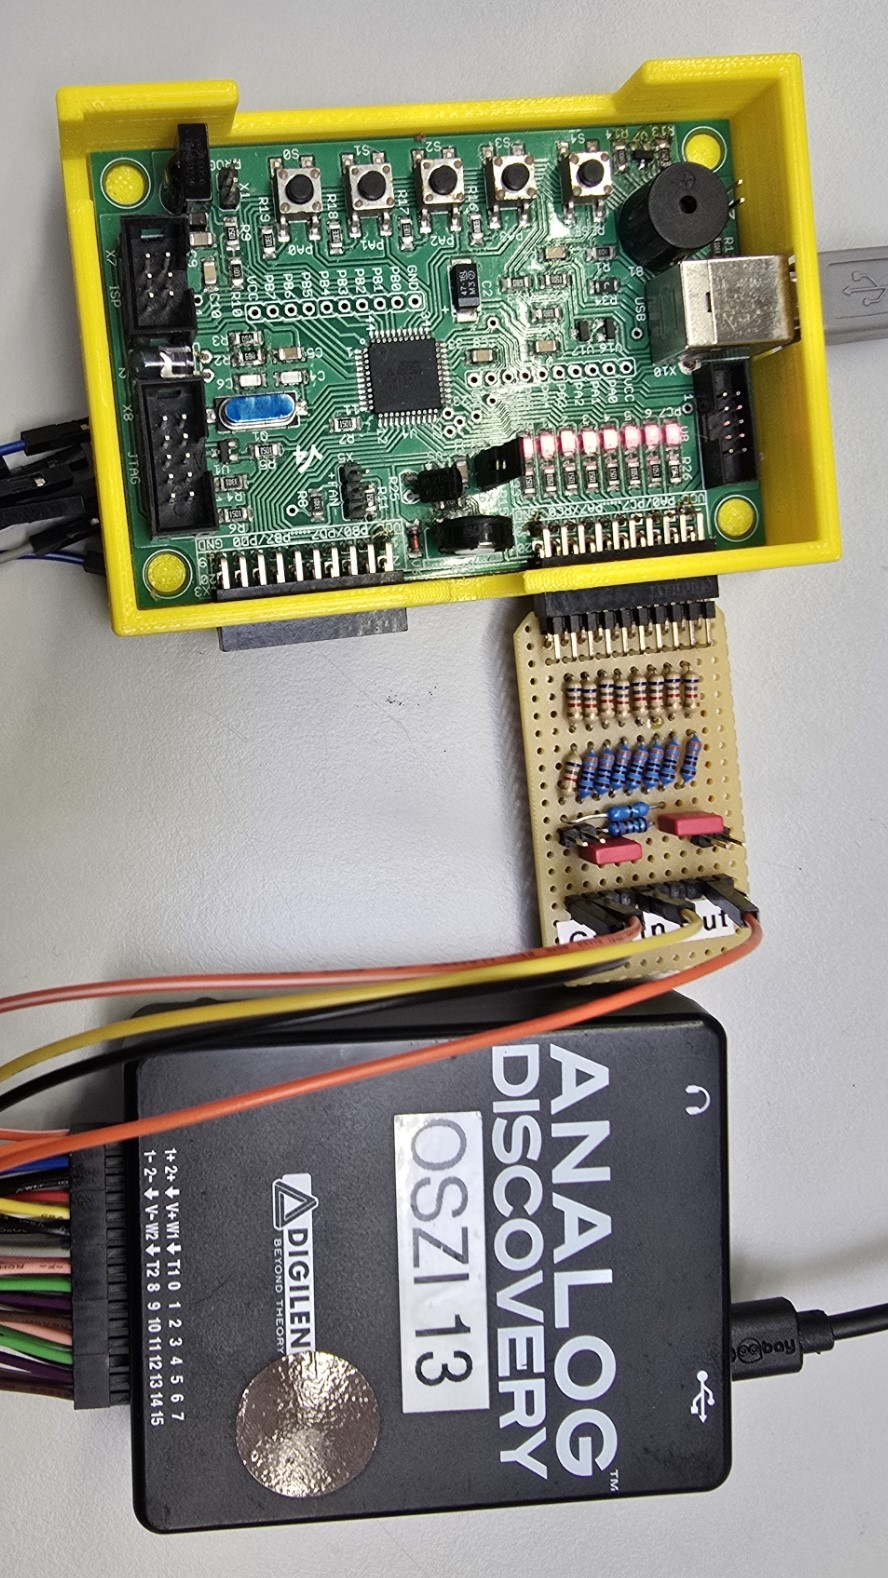
\includegraphics[width=0.5\linewidth, angle=90]{img/Aufbau_01.jpg}
        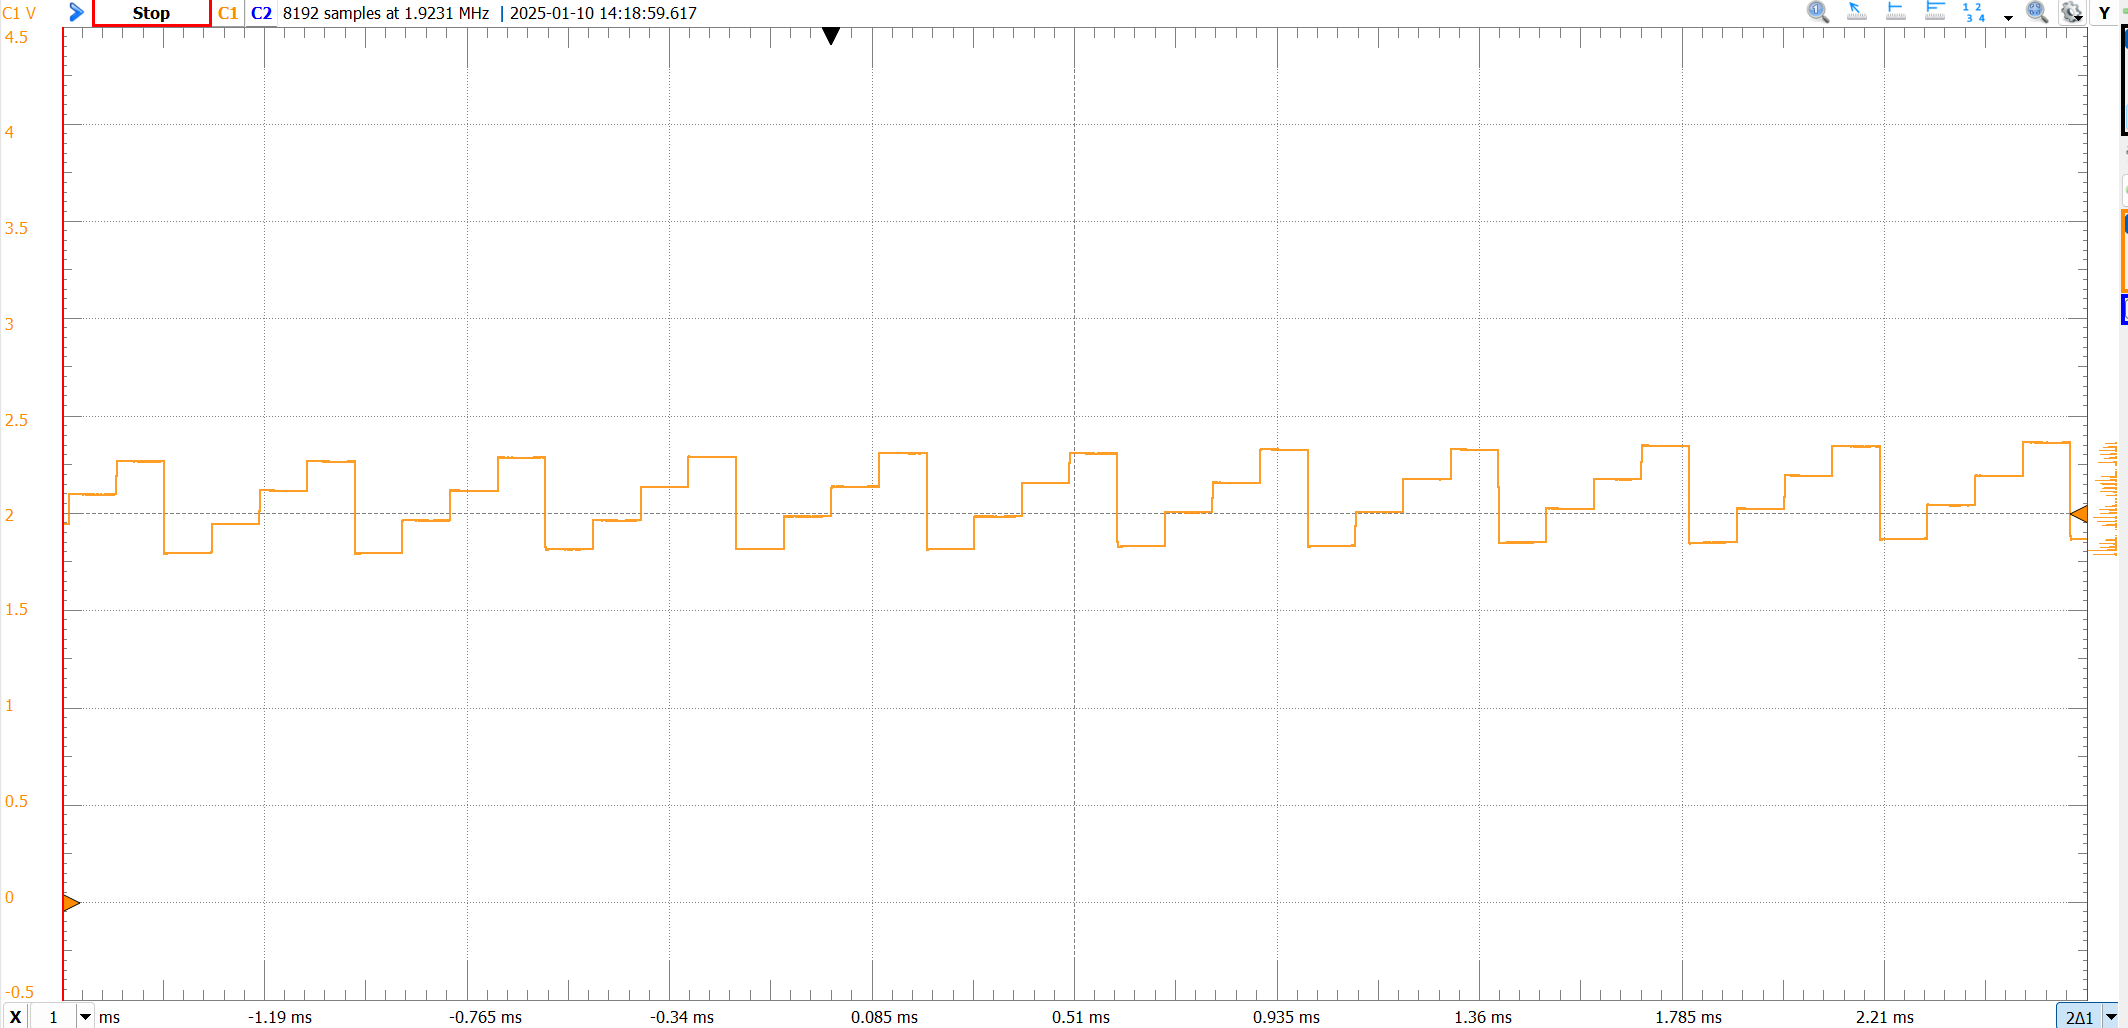
\includegraphics[width=0.9\linewidth]{img/Signal_07.png}
        \vspace{2cm}
    }\\
    \hline
\end{tabular}

\vspace{-1px}
\noindent
\begin{tabular}{|p{2.3cm}|p{1.8cm}|p{7.9cm}|p{2.5cm}|p{1.58cm}|}
    \vspace{0.1cm}Lehrer\vspace{0.2cm} & \vspace{0.1cm}\titellehrer & \vspace{0.15cm} \multirow{2}{7.1cm}{\centerline{Titel der Übung}\vspace{0.2cm}\newline\centerline{\huge \textbf{\titeltitel}}} & \vspace{0px} Übungsnummer & \vspace{1px}\titeluebungsnummer\\
    \cline{1-2}\cline{4-5}
    \vspace{0px}Geprüft\vspace{0.15cm} & \vspace{0px} \titelgeprueftdatum &  & \vspace{0px}Abgabe am\vspace{0.15cm} & \vspace{0px}\titelabgabedatum \\
    \hline
\end{tabular}
\newgeometry{top=2.5cm,left=2.5cm,right=2.5cm,bottom=2.5cm,headsep=0.3in,headheight=1in}

%Inhaltsverzeichnis
\pagestyle{fancy}
\tableofcontents
\newpage

%Begin der Dokumentation
\section{Übung 1 - Abtastung von Signalen}
\subsection{Analyse der ISR}
\begin{minted}{c}
ISR(TIMER0_COMP_vect) //fa=10kHz --> T=100us
{ 
	ue=ADCH;            //Einlesen des Samples
	ADCSRA|=(1<<ADSC);  //Start der neuen Messung
	
	ua=ue;              //Gibt Eingangssignal wieder aus
 
	PORTC=ua;           //Ausgabe des Samples
} 
\end{minted}
Zuerst wird die aktuelle Spannung des Eingangssignales gemessen, indem man das obere Byte des ADCs des ATMega16-Chips ausliest. Obwohl der ADC der MegaCard 10 Bits hat, werden nur die oberen 8 Bits verwendet.
Anschließend wird ein neuer Messzyklus des ADCs gestartet, indem man das ADSC-Bit im ADCSRA-Register setzt.
Das gemessene Eingangssignal (ue) wird anschließend auf das Ausgangssignal (ua) übertragen, ohne es zu verändern.
Schlussendlich wird das Ausgangssignal (ua) am Port C ausgegeben. An diesem ist ein R2R-DAC angeschlossen.

\subsection{Untersuchung des Samplingprozesses}
\subsubsection{Aufgabenstellung}
In dieser Aufgabe soll mit dem Analog Discovery ein Sinussignal mit einer Frequenz von 200Hz, einer Amplitude von 2V und einem DC-Offset von 2V in die MegaCard eingespeist werden. Das entstehende Ausgangssignal soll untersucht werden und die Spannung des niedrigsten Bits ($U_{LSB}$) und die Frequenz des Samplingprozesses ($f_A$) sollen erfasst werden.

\subsubsection{Schaltungsaufbau}
\begin{figure}[h]
    \centering
    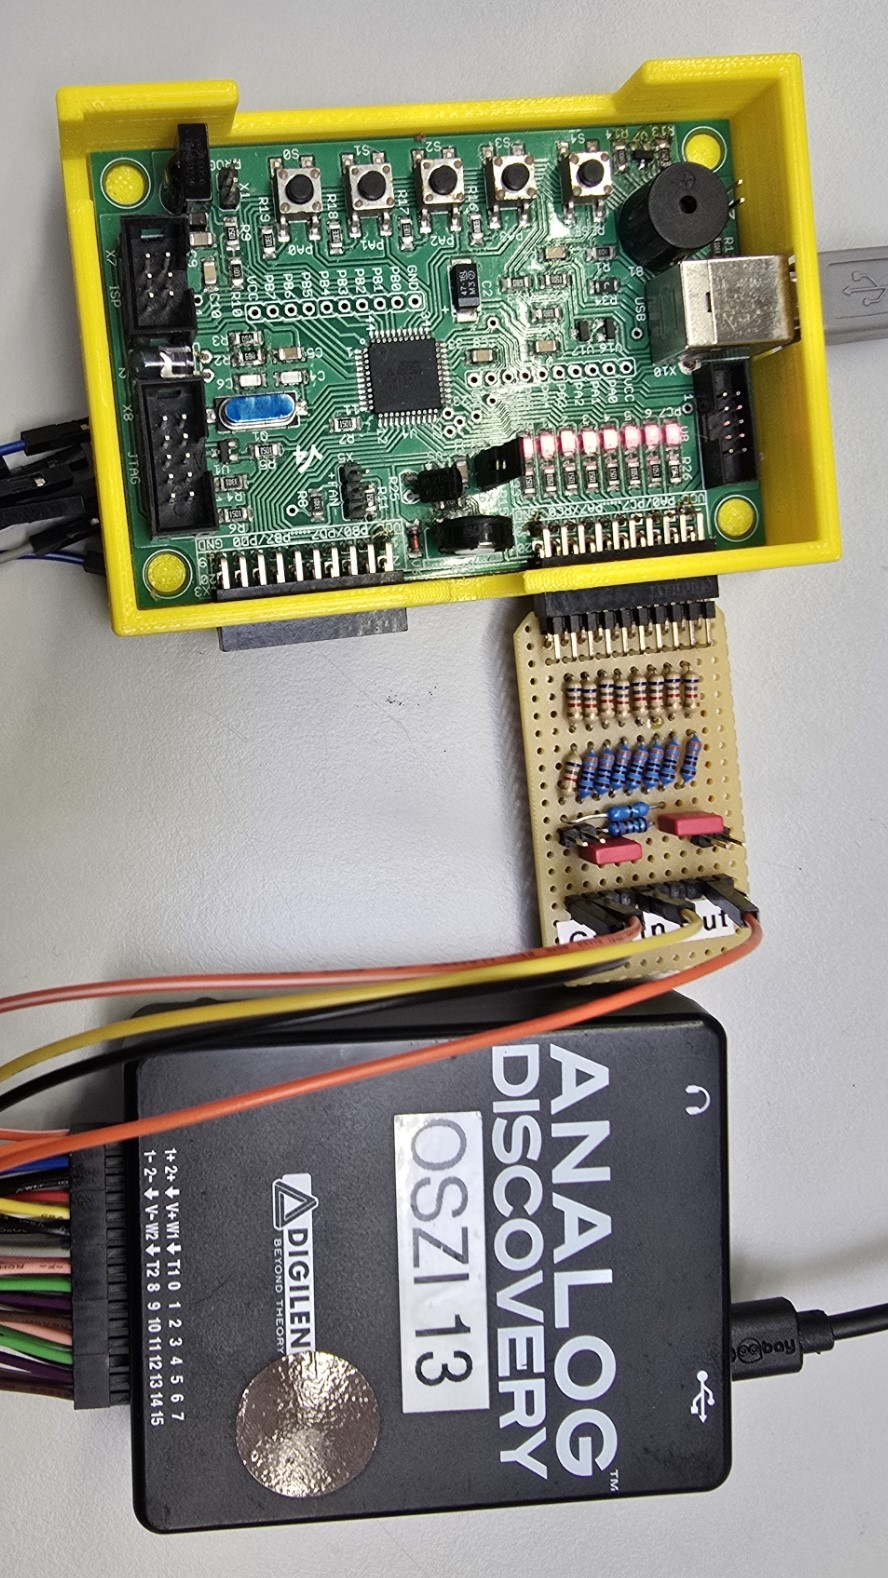
\includegraphics[angle=90,width=0.8\linewidth]{img/Aufbau_01.jpg}
\end{figure}

\newpage
\subsubsection{Ausgangssignal}
\begin{figure}[h]
    \centering
    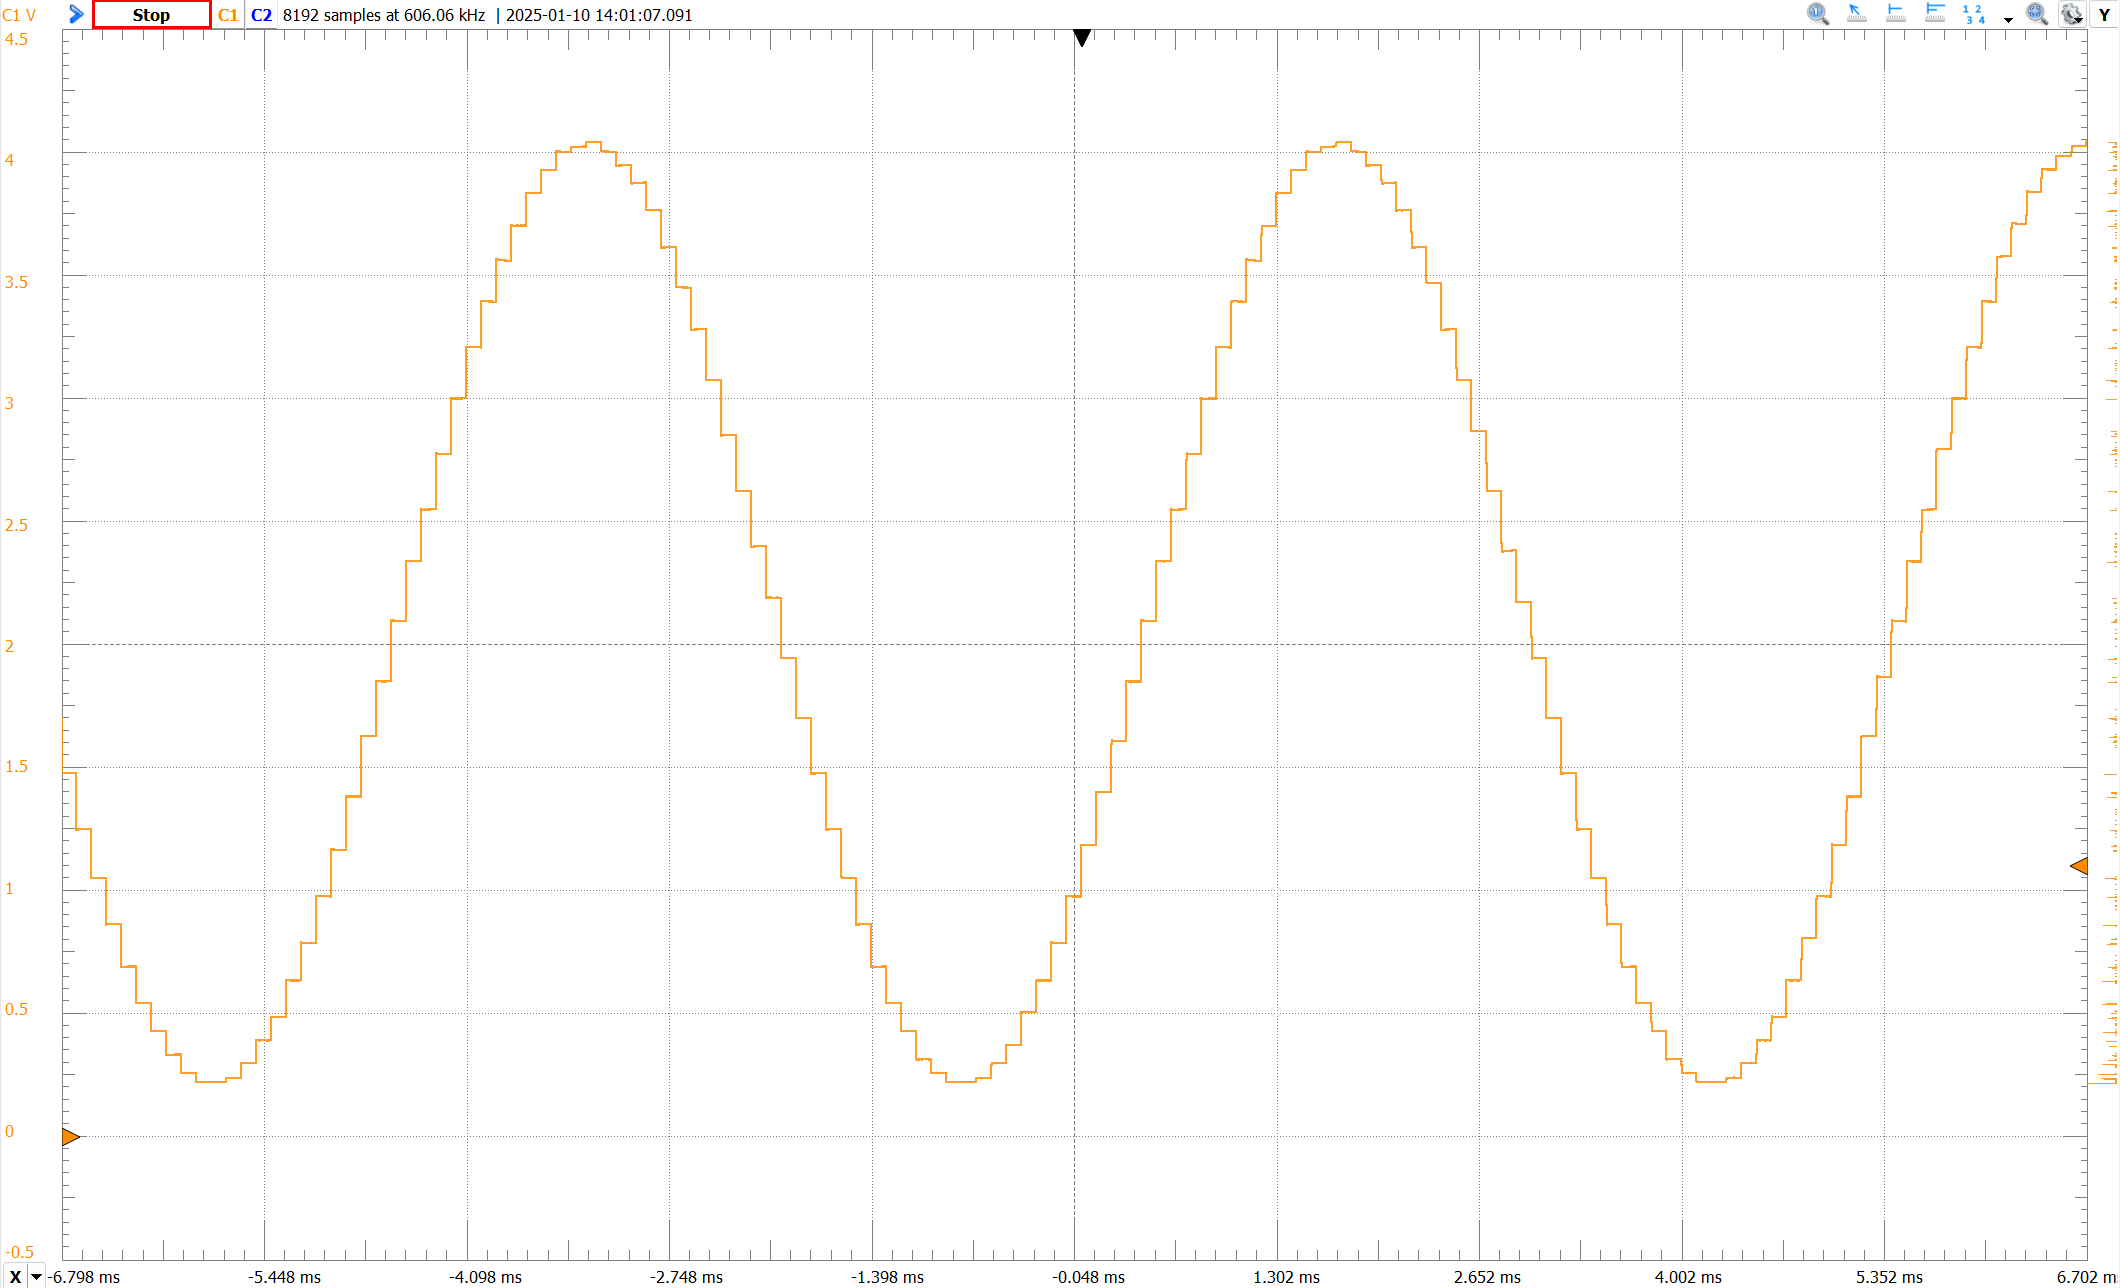
\includegraphics[width=1\linewidth]{img/Signal_01.png}
\end{figure}
\newpage
\subsubsection{Spannungsauflösung}
\paragraph{Theroretischer Wert}\mbox{}\\
\begin{math}
    U_B=5V\\
    n=8\\
    \\
    U_{LSB}=\frac{U_B}{2^n}=\underline{19.831mV}
\end{math}

\paragraph{Messung}\mbox{}\\
Um die Spannungsauflösung des DACs zu bestimmen, muss man am Tiefpunkt des Sinussignales messen, da dort die Spannung nur langsam steigt und somit sichergestellt wird, dass nur ein Bit gemessen wird. Hier wurde ein Wert von \textbf{20.309mV} erhalten.
\begin{figure}[h]
    \centering
    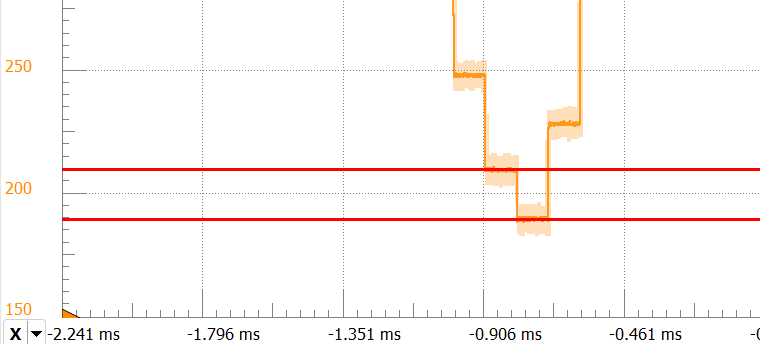
\includegraphics[width=0.8\linewidth]{img/Messung_Signal_01.png}
    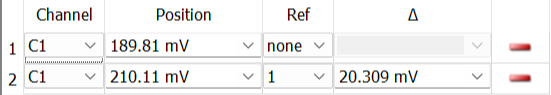
\includegraphics[width=0.8\linewidth]{img/Messung_01.png}
\end{figure}

\paragraph{Vergleich}\mbox{}\\
Wenn man den theoretischen Wert mit dem gemessenen vergleicht, unterscheiden sich diese um nur 777.75µV. Dies stammt von der Toleranz der Eingangsspannung (5V vom USB) und der Ungenauigkeit der Messung.

\subsubsection{Samplingfrequenz}
\paragraph{Theroretischer Wert}\mbox{}\\
\begin{math}
    F_{CPU}=12MHz\\
    OCR0=149\\
    \\
    f_a=\frac{F_{CPU}}{8\cdot (OCR0+1)}=\underline{10kHz}\\
\end{math}

\newpage
\paragraph{Messung}\mbox{}\\
Die Samplingfrequenz muss am Nulldurchgang des Eingangssignales erfasst werden, da sich die Werte des Eingangssignales (Sinus) dort sehr schnell ändern und die benötigten Punkte leichter erkennbar sind.
\begin{figure}[h]
    \centering
    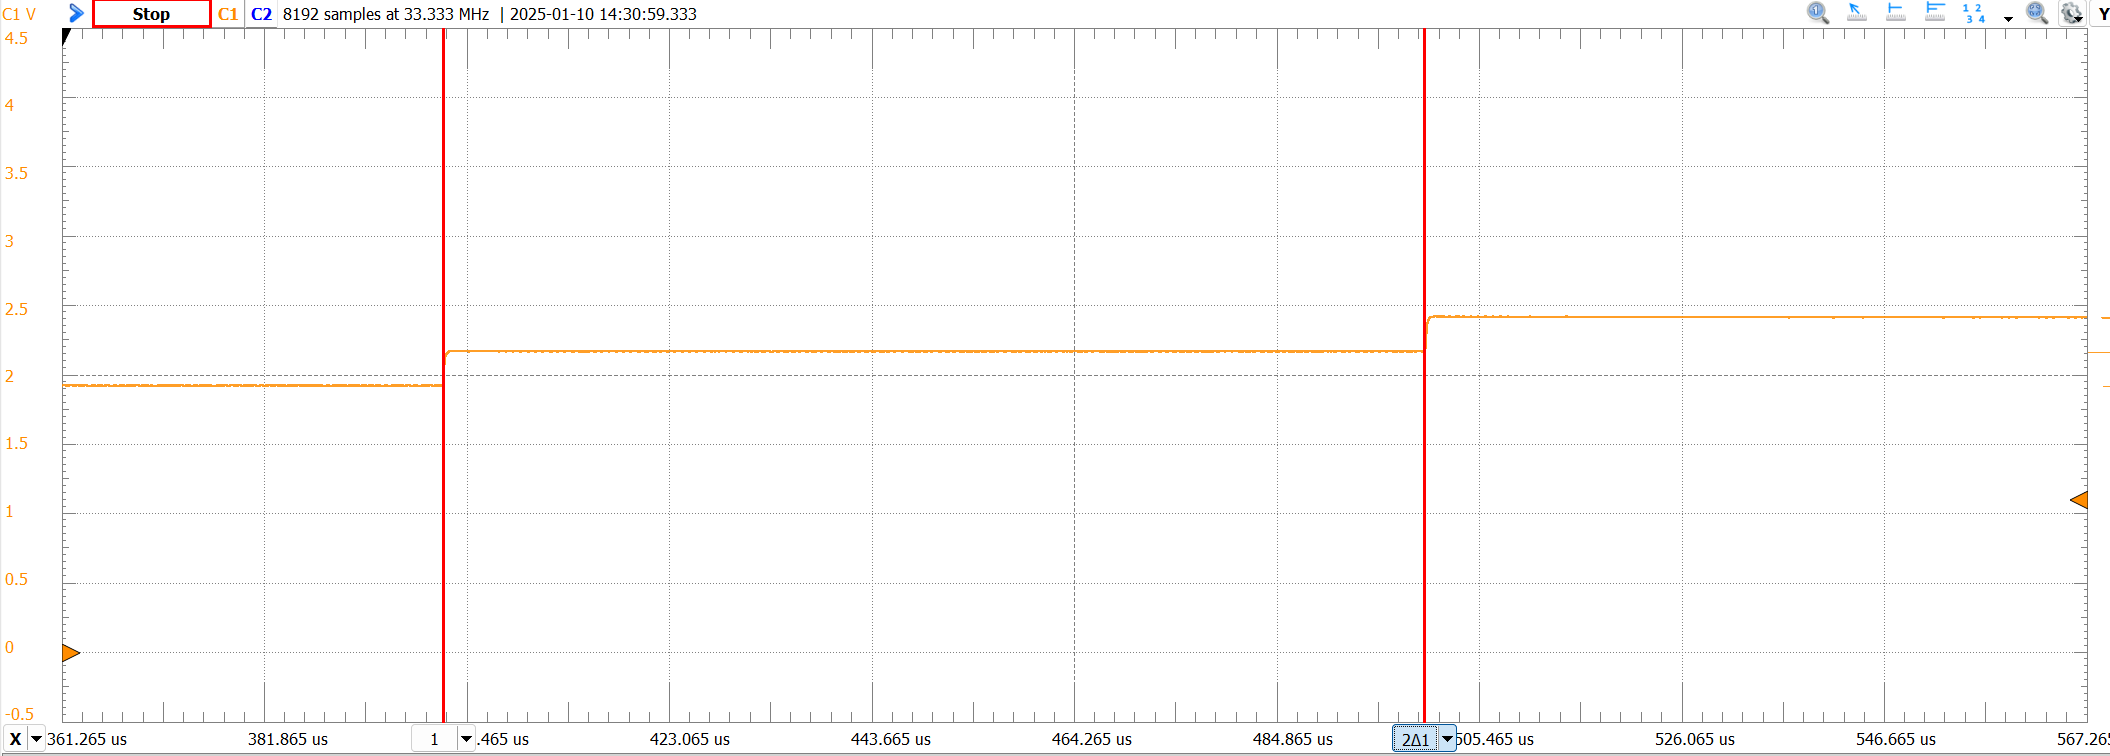
\includegraphics[width=0.75\linewidth]{img/Messung_Signal_02.png}
    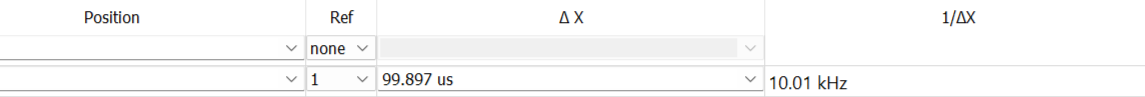
\includegraphics[width=0.75\linewidth]{img/Messung_02.png}
\end{figure}

\paragraph{Vergleich}\mbox{}\\
Wenn man den theoretischen Wert mit dem gemessenen vergleicht, unterscheiden sich diese um nur 10Hz. Diese Ungenauigkeit stammt von der Ungenauigkeit des Quarzes der Megacard, welcher den Timer zum Ausführen der Messung steuert, und der Toleranz des Analog Discoverys. 

\subsection{Untersuchung des Rekonstruktionsfilters}
\subsubsection{Aufgabenstellung}
In dieser Aufgabe soll der Rekonstruktionsfilter des DACs über den Jumper X2 eingeschalten werden. Das entstehende Ausgangssignal soll mit der vorherigen Aufgabe (ohne Rekonstruktionsfilter) verglichen werden.
\subsubsection{Ausgangssignal}
\begin{figure}[h]
    \centering
    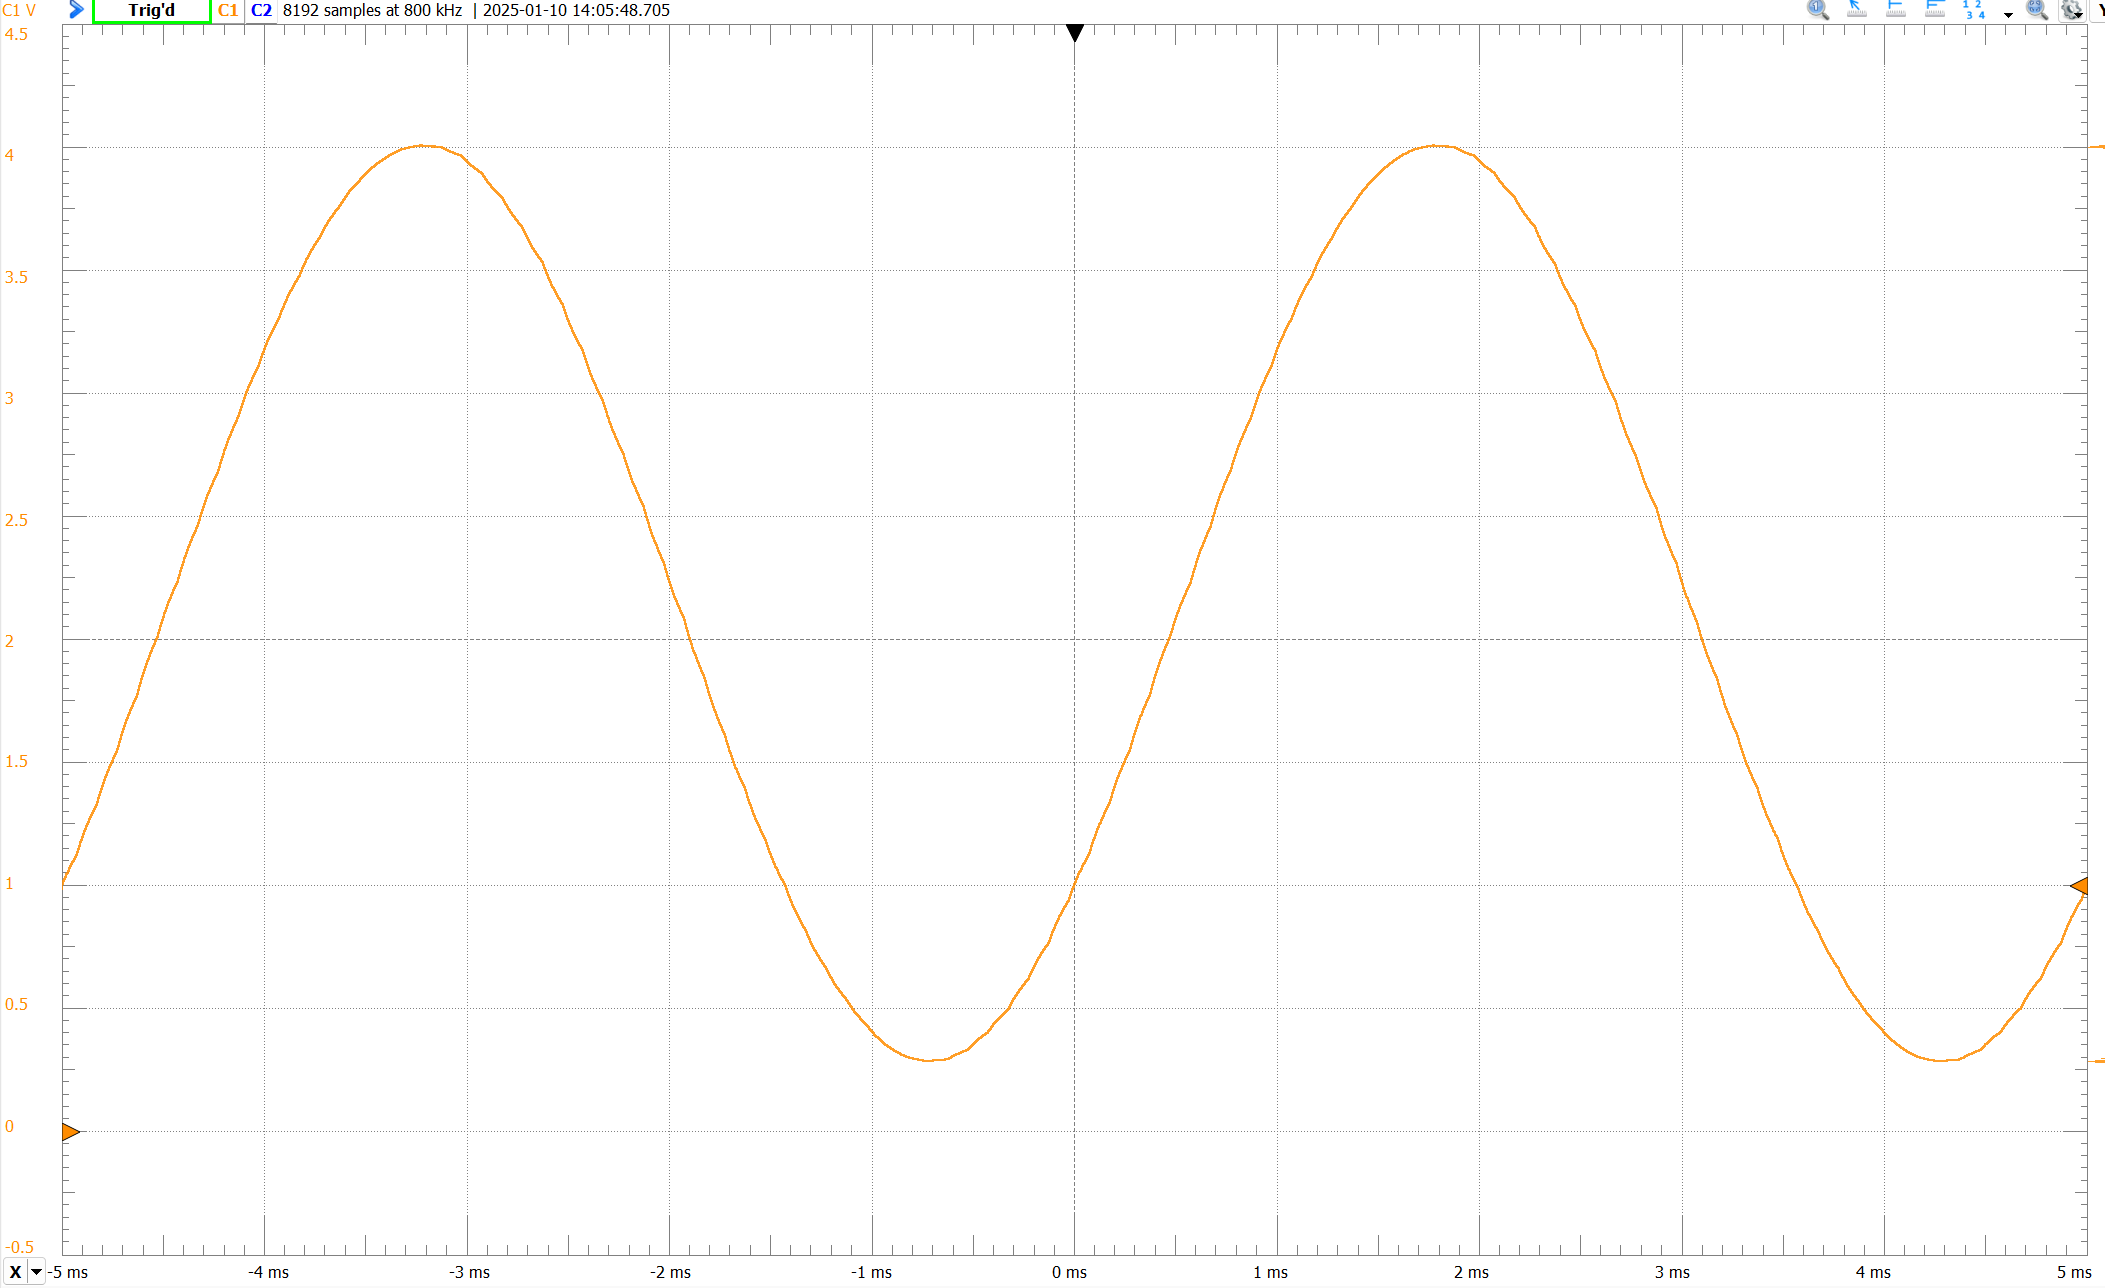
\includegraphics[width=0.6\linewidth]{img/Signal_03.png}
\end{figure}

\subsubsection{Vergleich}
Beim Vergleichen der beiden Ausgangssignale ist schnell erkennbar, dass das Rekonstruktionsfilter die hohen Frequenzen des Signals wegfiltert. Dies ist erkennbar, da das Signal nicht mehr stufenartig aufgebaut ist. Somit ähnelt es einem reinen Sinus mehr als dem Ausgangssignal ohne den Filter.
\newpage
\subsection{Untersuchung mehrerer Frequenzen}
\subsubsection{Aufgabenstellung}
In dieser Aufgabe sollen mehrere Signalfrequenzen angelegt werden. Dabei soll kein Filter des DACs aktiviert werden. Die zu messenden Frequenzen sind 2kHz, 5kHz, 8kHz, 10kHz und 12kHz. Dabei ist der Zeit- und Frequenzbereich zu untersuchen.

\subsubsection{2kHz}
\paragraph{Zeitbereich}\mbox{}\\
Das Signal im Zeitbereich hat zwar wenig Ähnlichkeit mit einem Sinus, aber seine Form ist immer noch erkennbar. Dies stammt von der langsamen Abtastfrequenz im Vergleich zum Eingangssignal.
\begin{figure}[h]
    \centering
    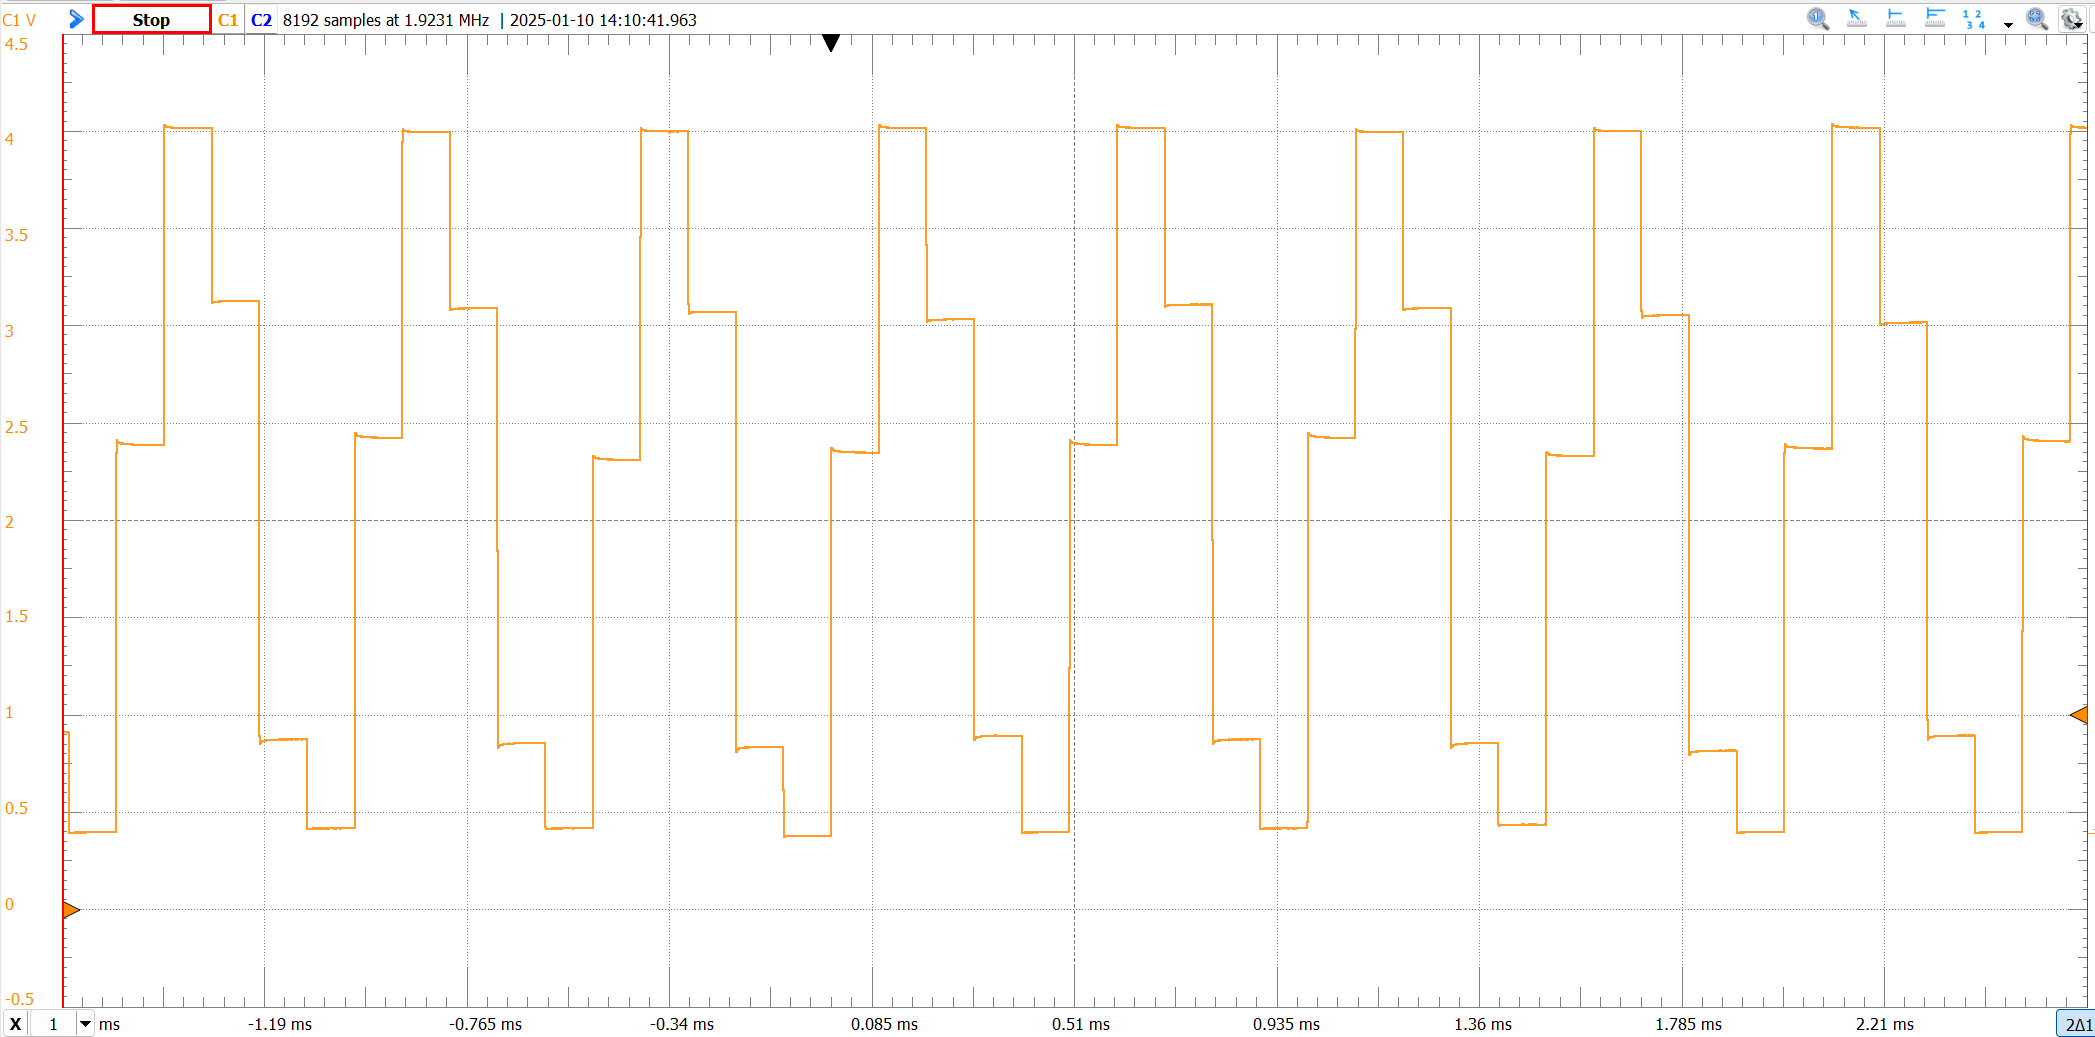
\includegraphics[width=0.75\linewidth]{img/Signal_04.png}
\end{figure}

\paragraph{Frequenzbereich}\mbox{}\\
Im Frequenzbereich des Signals kann ein hoher Peak alle 2kHz erkannt werden. Dabei sind die bei 2kHz- und 10kHz-Peaks am höchsten. Der 2kHz-Peak stammt vom Eingangssignal, welches eine Frequenz von 2kHz hat. Der Peak bei 8kHz stammt vom Samplingprozess, da das Signal mit einer Frequenz von 10kHz aufgenommen wird, wird es auf 8kHz (10kHz-2kHz) und 12kHz (10kHz+2kHz) gespiegelt.
\begin{figure}[h]
    \centering
    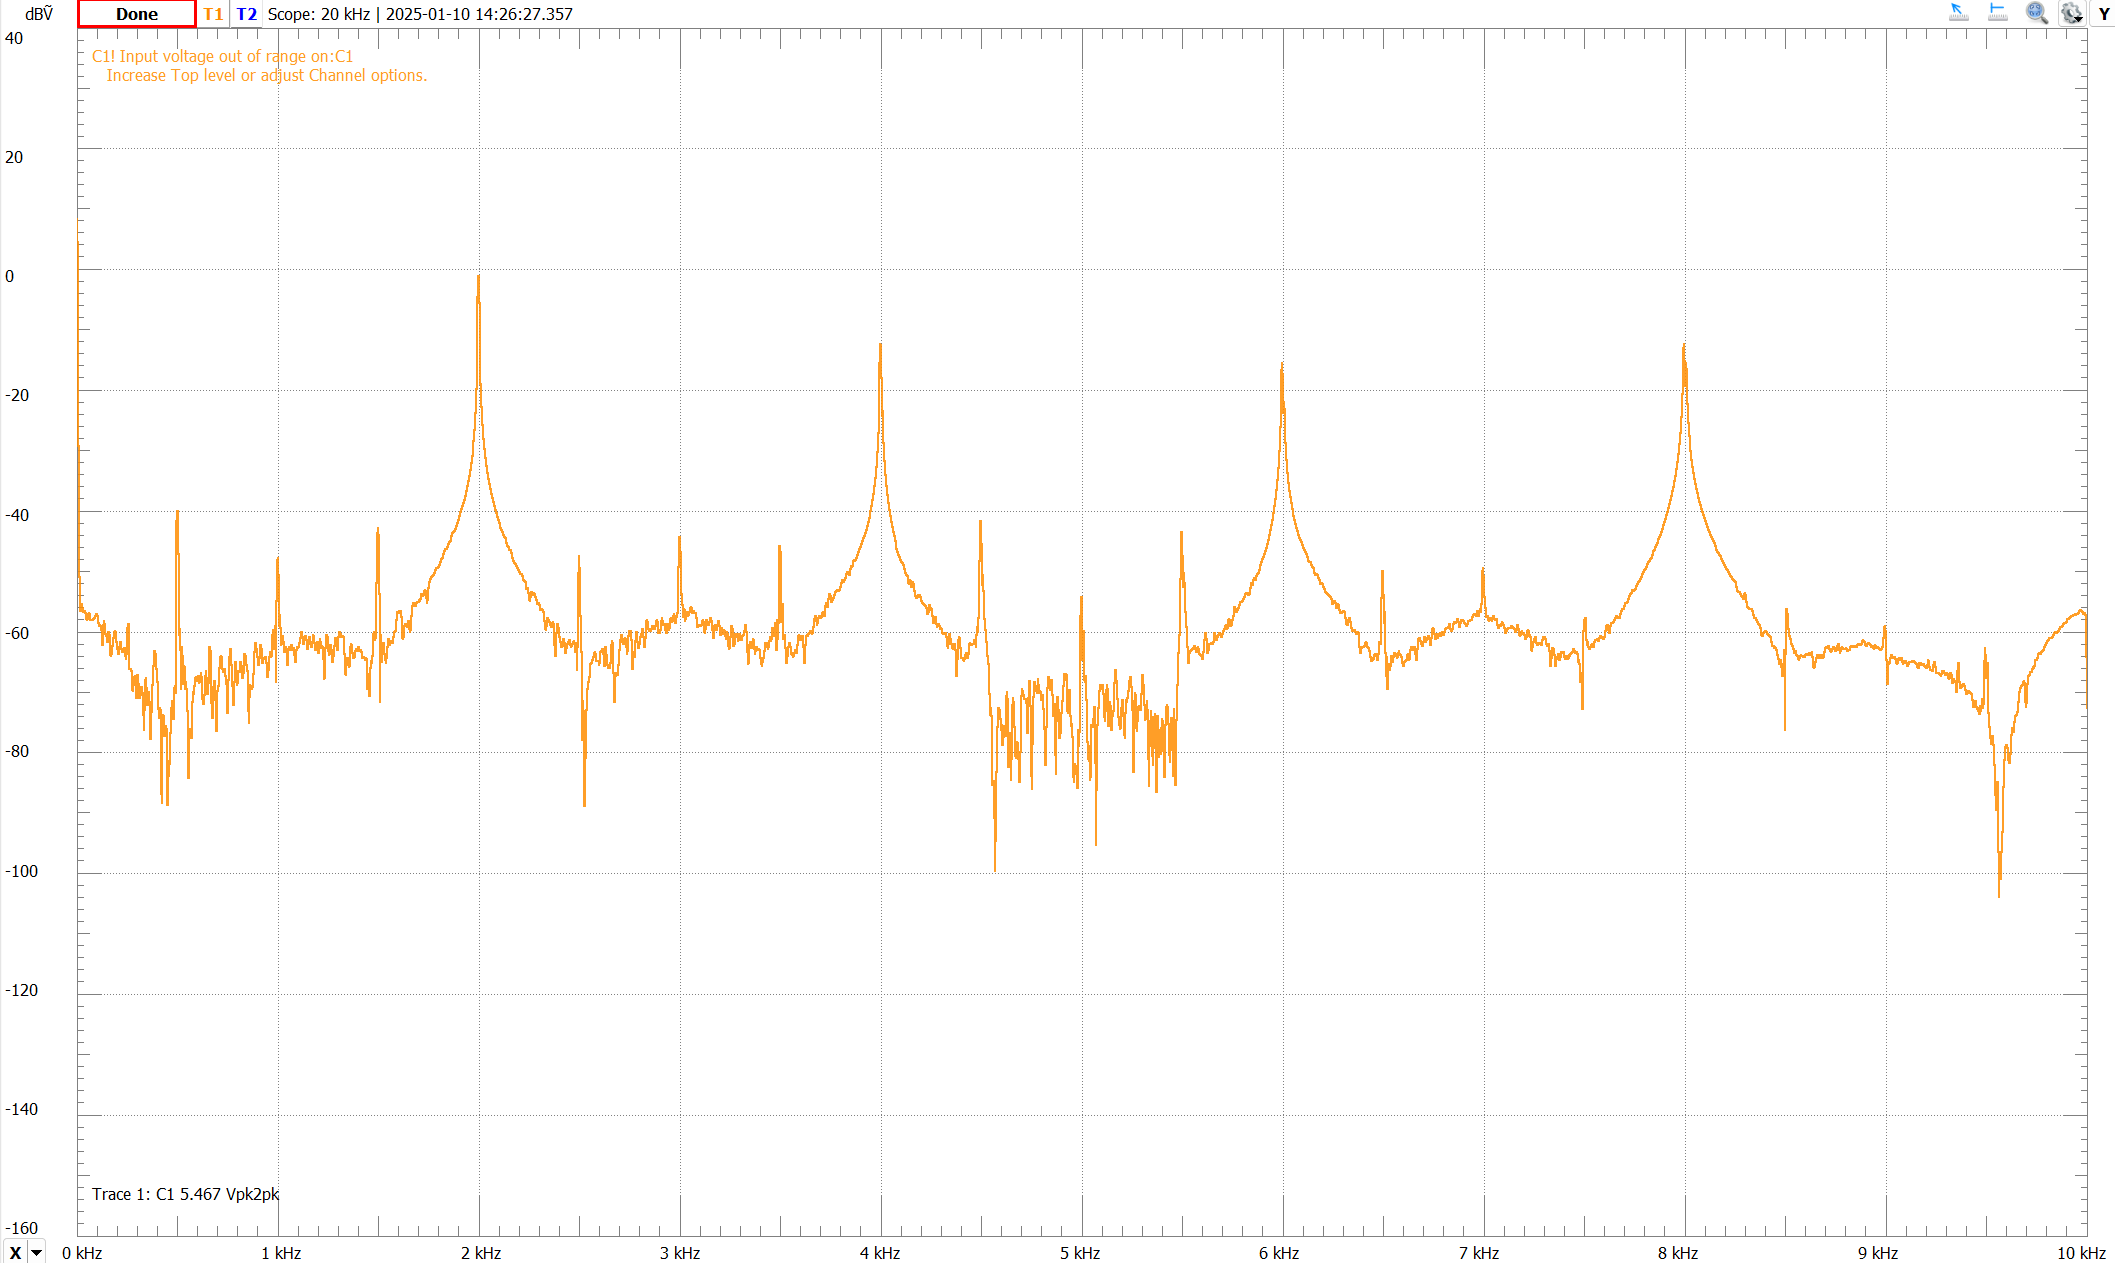
\includegraphics[width=0.75\linewidth]{img/Freq_04.png}
\end{figure}

\newpage
\subsubsection{5kHz}
\paragraph{Zeitbereich}\mbox{}\\
Das Signal im Zeitbereich hat keine Ähnlichkeit mit einem Sinus, sondern sieht wie ein Rechtecksignal aus. Das angezeigte Signal verändert zudem seine Amplitude über die Zeit. Dies liegt daran, dass die Nyquist-Frequenz erreicht wurde. Aus diesem Grund werden zu wenig Messpunkte des Eingangssignals aufgenommen und verarbeitet, was zu dem rechteckförmigen Aufbau führt. Die Amplitudenänderung des Ausgangssignals stammt von leichten Frequenzdifferenzen zwischen dem Eingangssignal und der Samplingfrequenz, die dazu führen, dass die Messpunkte immer an anderen Stellen des Sinussignals aufgenommen werden.
\begin{figure}[h]
    \centering
    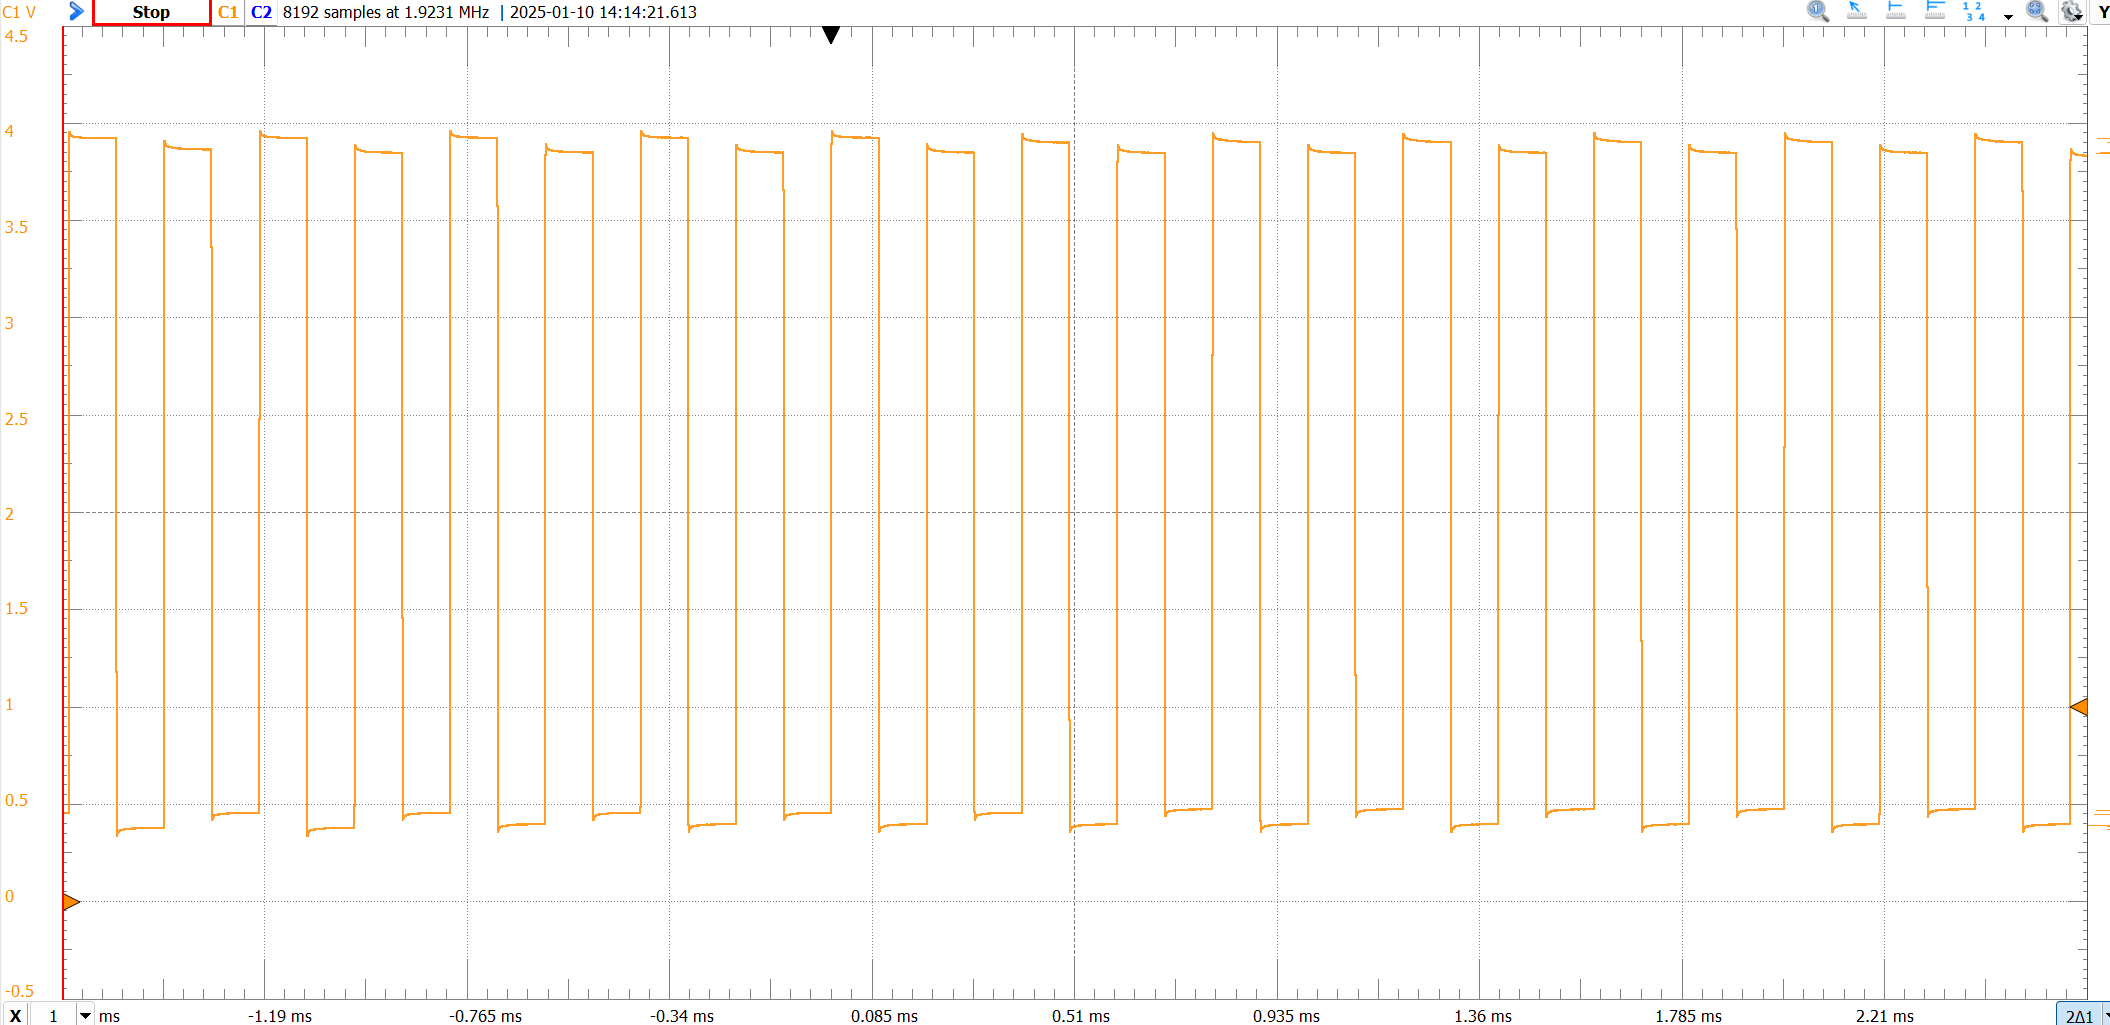
\includegraphics[width=0.8\linewidth]{img/Signal_05.png}
\end{figure}

\paragraph{Frequenzbereich}\mbox{}\\
Im Frequenzbereich des Signals kann ein hoher Peak bei 5 kHz und 15 kHz erkannt werden. Das Signal bei 5kHz ist die Summe aus dem Eingangssignal und der unteren Spiegelung bei der Samplingfrequenz (10kHz - 5kHz). Der Peak bei 15kHz stammt von der oberen Spiegelung bei der Samplingfrequenz (10kHz + 5kHz).
\begin{figure}[h]
    \centering
    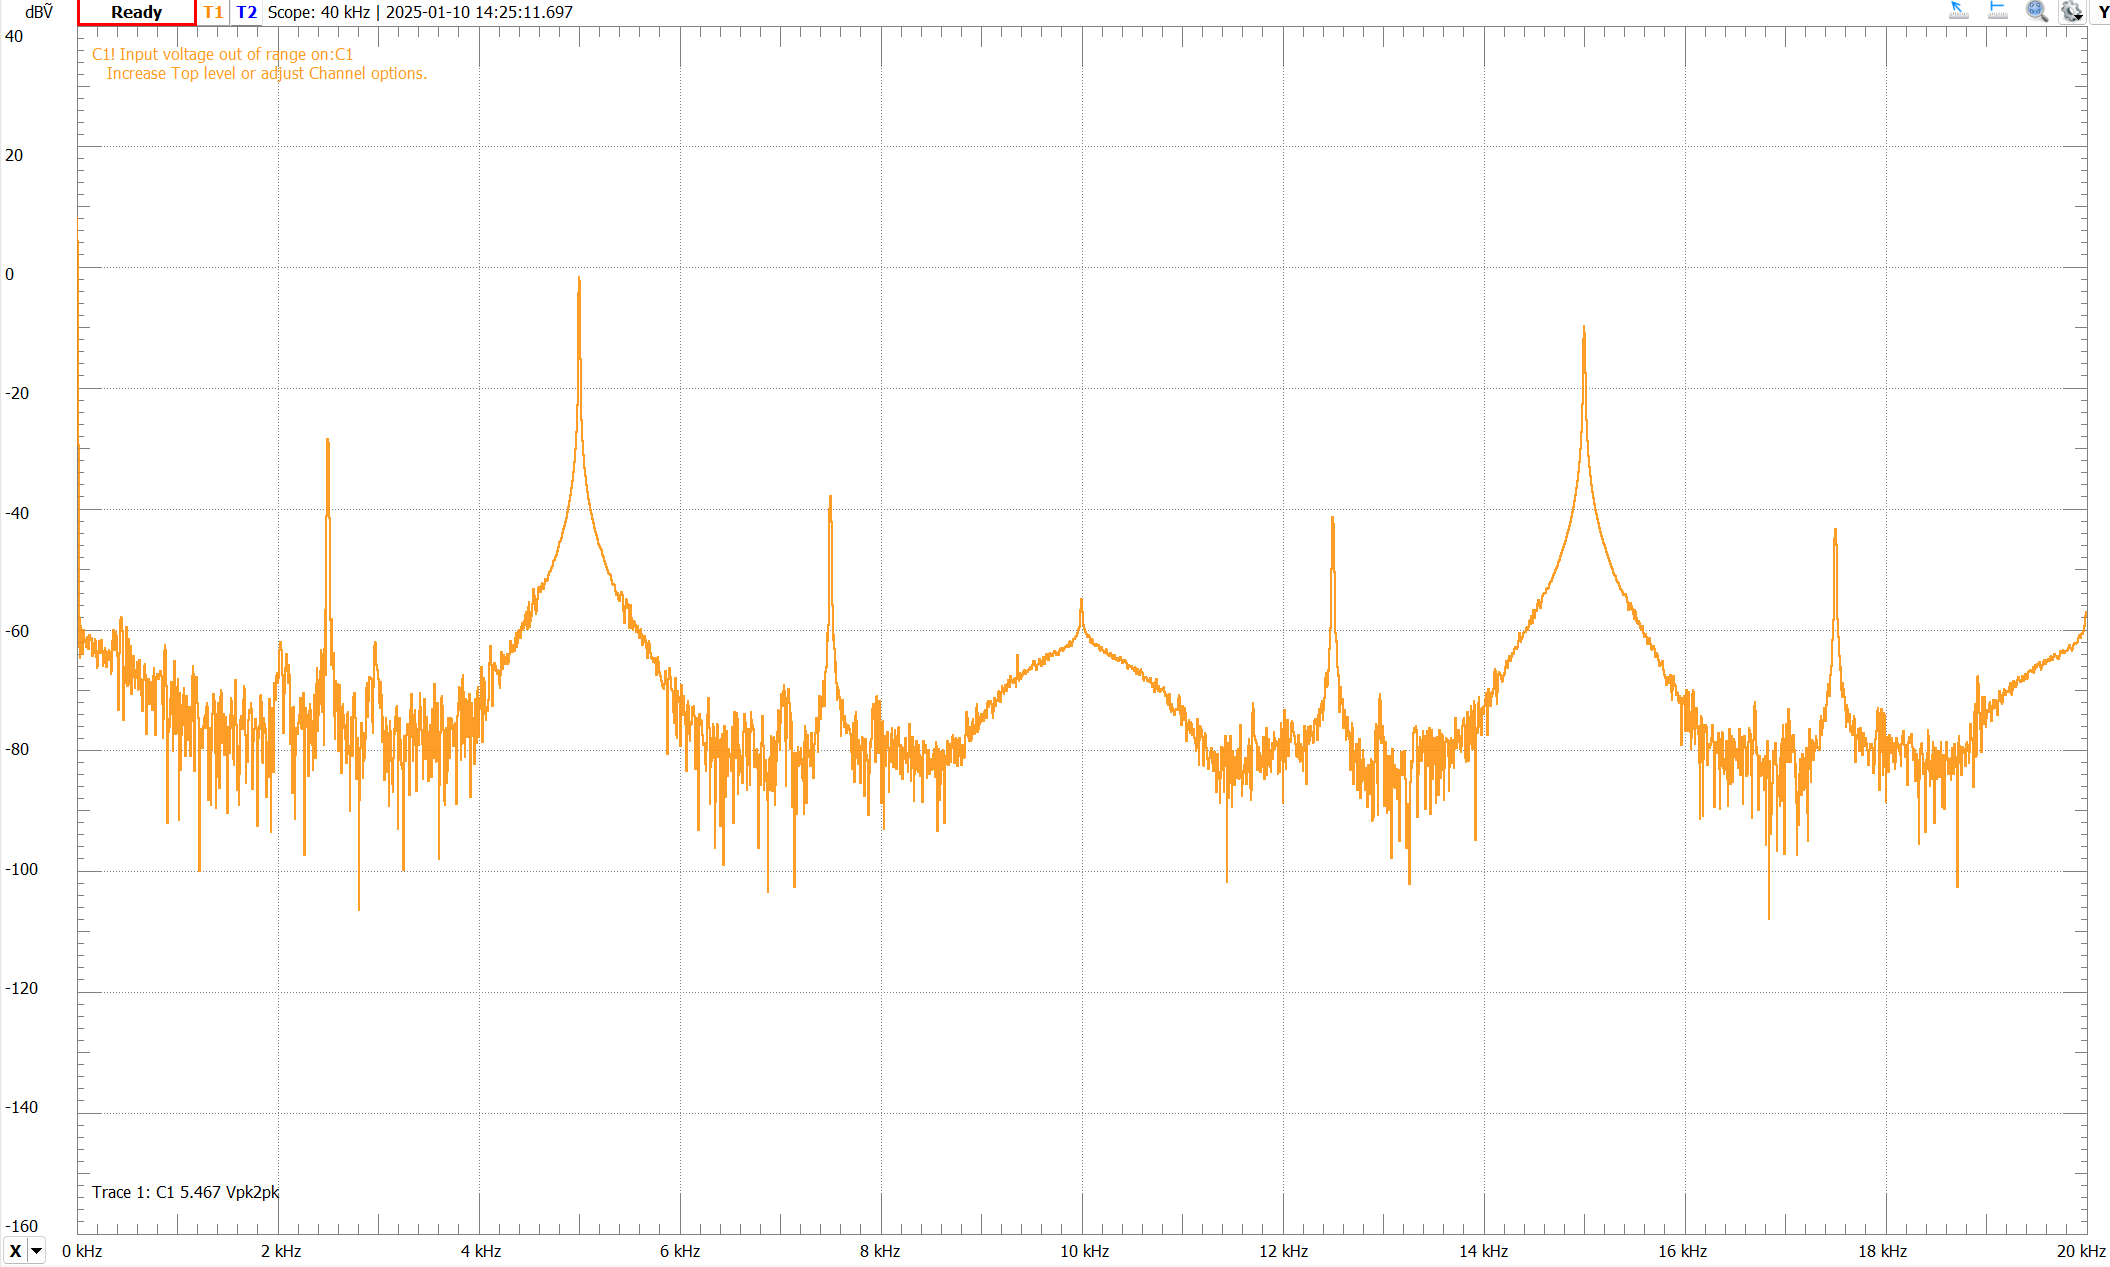
\includegraphics[width=0.8\linewidth]{img/Freq_05.png}
\end{figure}

\subsubsection{8kHz}
\paragraph{Zeitbereich}\mbox{}\\
Bei der Untersuchung des Signales im Zeitbereich ist schnell erkennbar, dass es dem Signal bei einer Eingangsfrequenz von 2kHz sehr ähnlich ist. Dies liegt daran, dass die Eingangsfrequenz des 2kHz-Signals mit der unteren Spiegelung des 8kHz bei einer Samplingfrequenz von 10kHz ist (10kHz - 8kHz = 2kHz). Die untere Spiegelung des 2kHz-Signals (8kHz) wird durch das Eingangssignal ersetzt. Dies ist bei den anderen Punkten des Signales auch der Fall.
\begin{figure}[h]
    \centering
    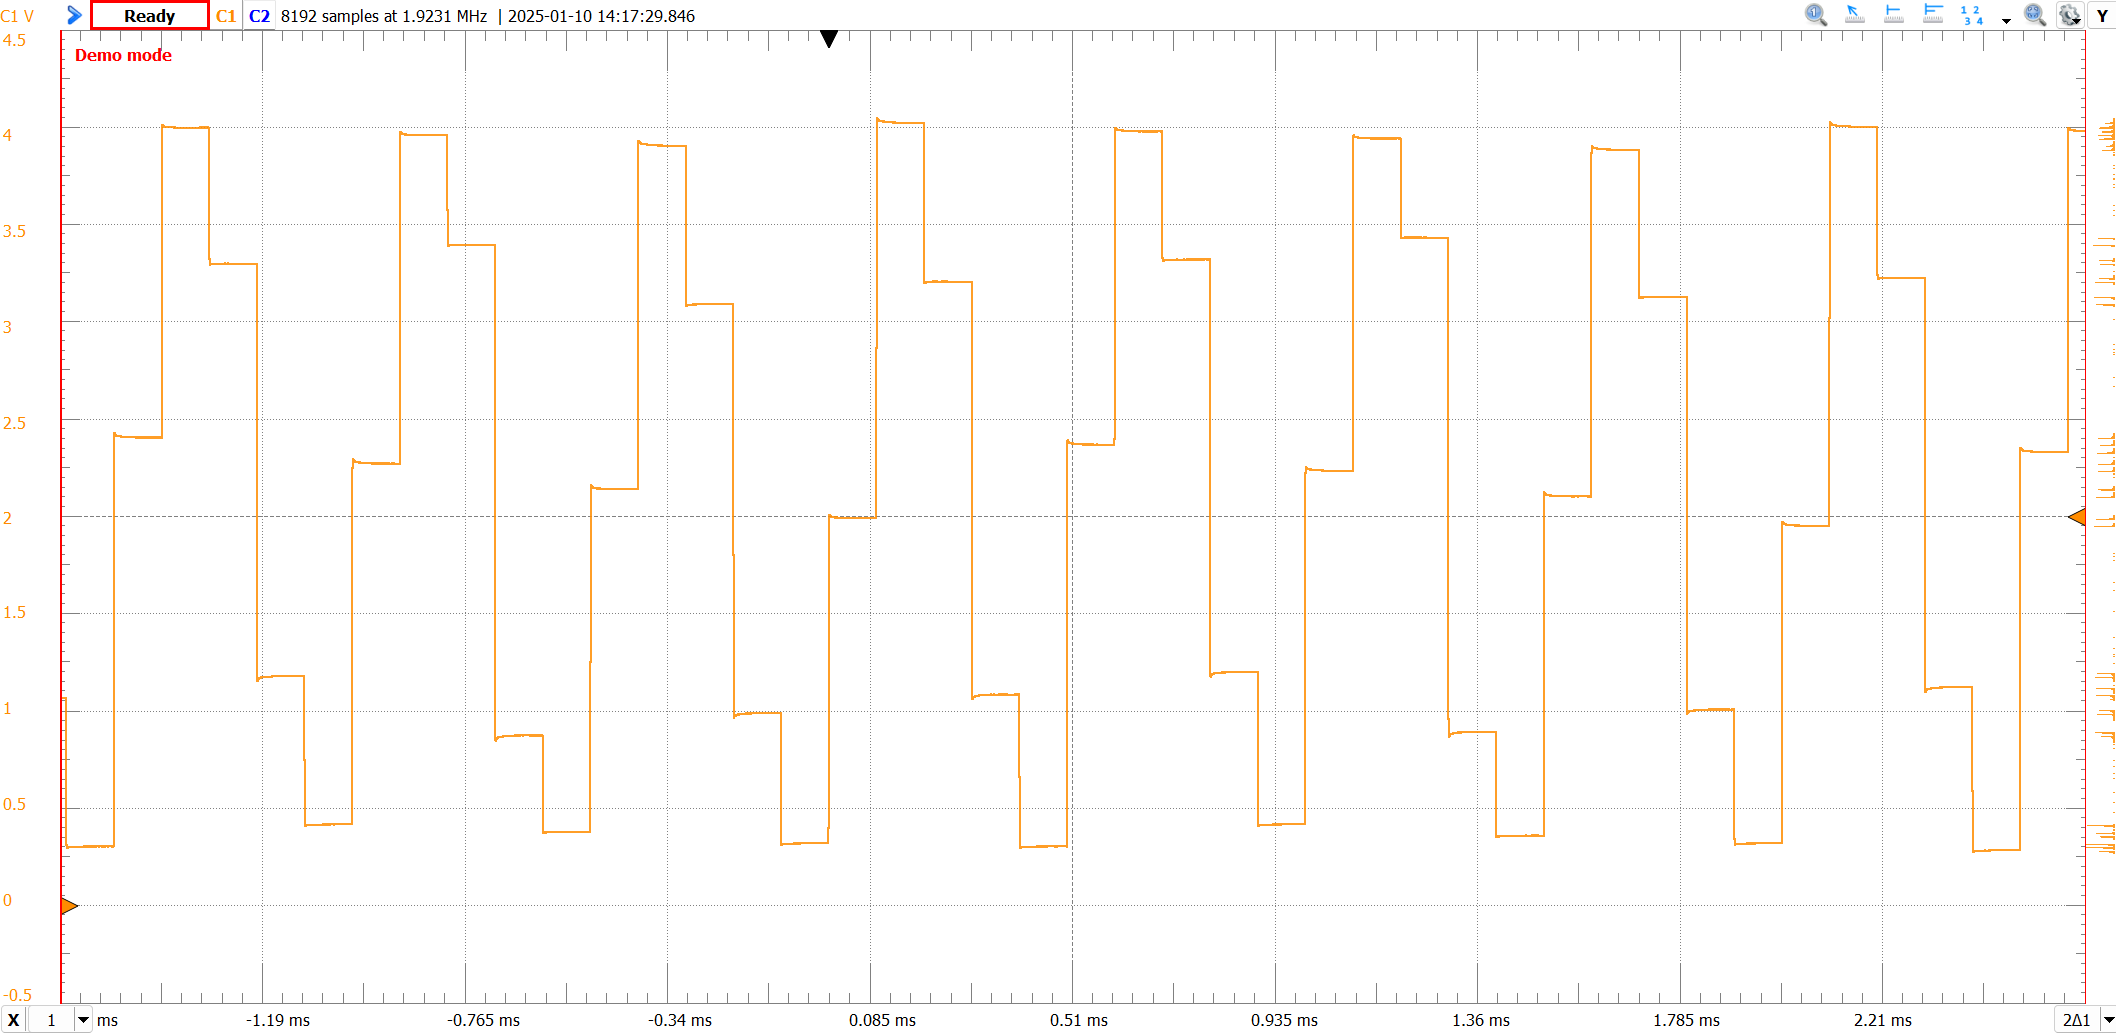
\includegraphics[width=0.8\linewidth]{img/Signal_06.png}
\end{figure}


\paragraph{Frequenzbereich}\mbox{}\\
Im Frequenzbereich kann erneut die Ähnlichkeit mit dem des 2kHz-Eingangssignals erkannt werden. Der Grund dafür wurde unter dem Punkt \textit{Zeitbereich} erklärt. Es sind erneut zwei Peaks bei 2kHz- und 10kHz zu erkennen. Der 2kHz-Peak stammt von der Reflektion durch die Samplingfrequenz (10kHz - 8kHz). Der Peak bei 8kHz stammt vom Eingangssignal.
\begin{figure}[h]
    \centering
    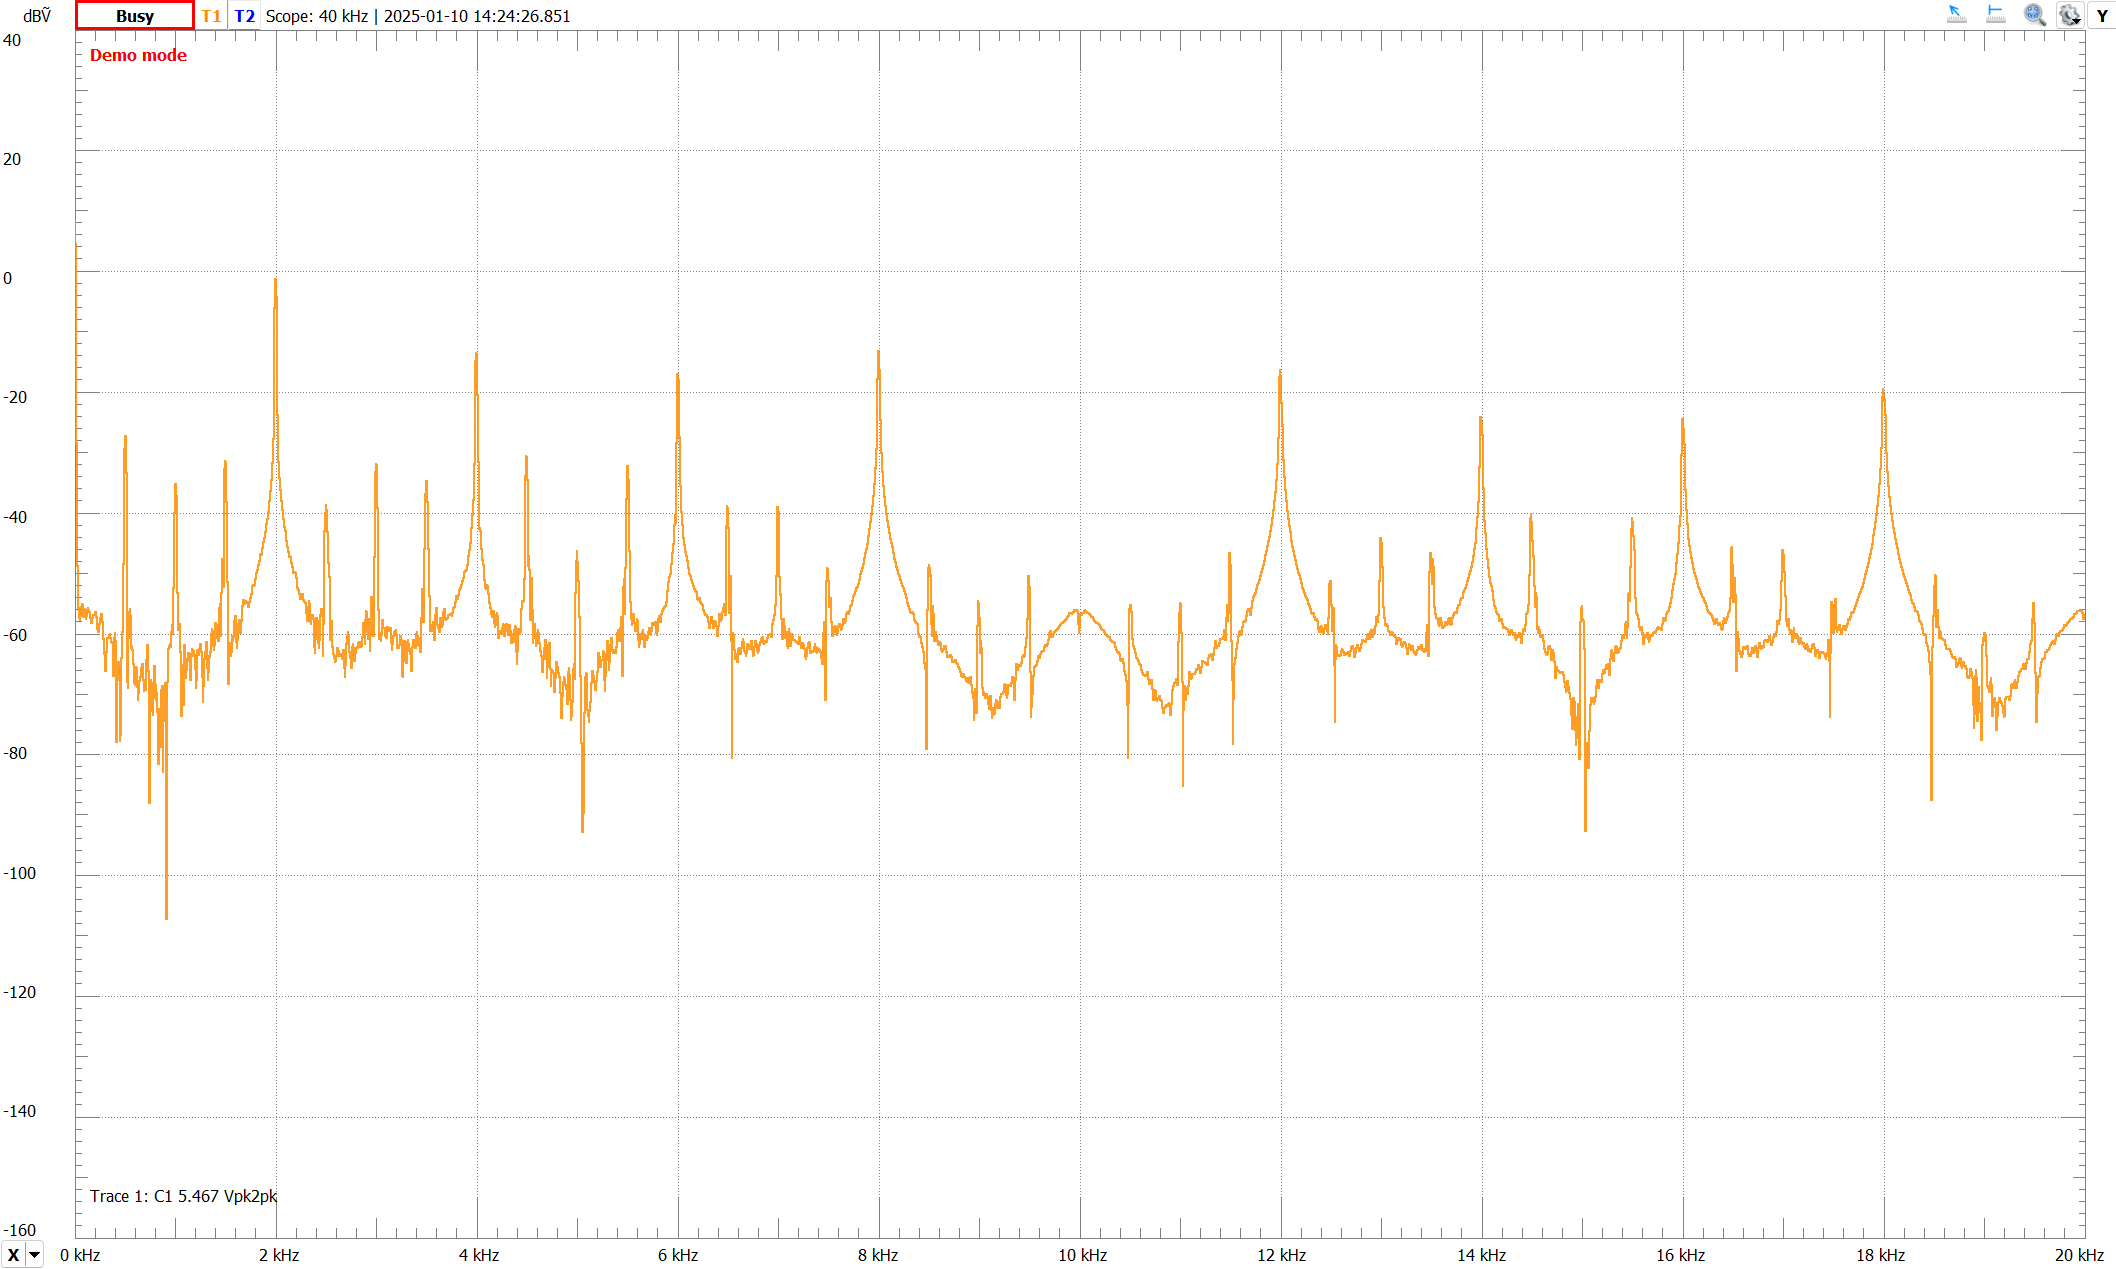
\includegraphics[width=0.8\linewidth]{img/Freq_06.png}
\end{figure}

\subsubsection{10kHz}
\paragraph{Zeitbereich}\mbox{}\\
Das Signal im Zeitbereich hat keine Ähnlichkeit mit einem Sinus, sondern sieht wie ein Sägezahn aus. Dieses verändert seine Höhe und seine Richtung (Spiegelung entlang der y-Achse). Zudem ist die Amplitude des Ausgangssignals sehr viel kleiner als bei den Messungen mit den anderen Frequenzen und wie das Eingangssignal. Die Form des Ausgangssignals stammt von der hohen Frequenz des Eingangssignals im Vergleich zur Samplingfrequenz. Theoretisch sollte das Signal eine DC-Spannung darstellen, da der Sinus am Eingang immer an den gleichen Punkten abgemessen wird. Durch leichte Toleranzen der Frequenzen wird dies nicht am Ausgangssignal beobachtet.
\begin{figure}[h]
    \centering
    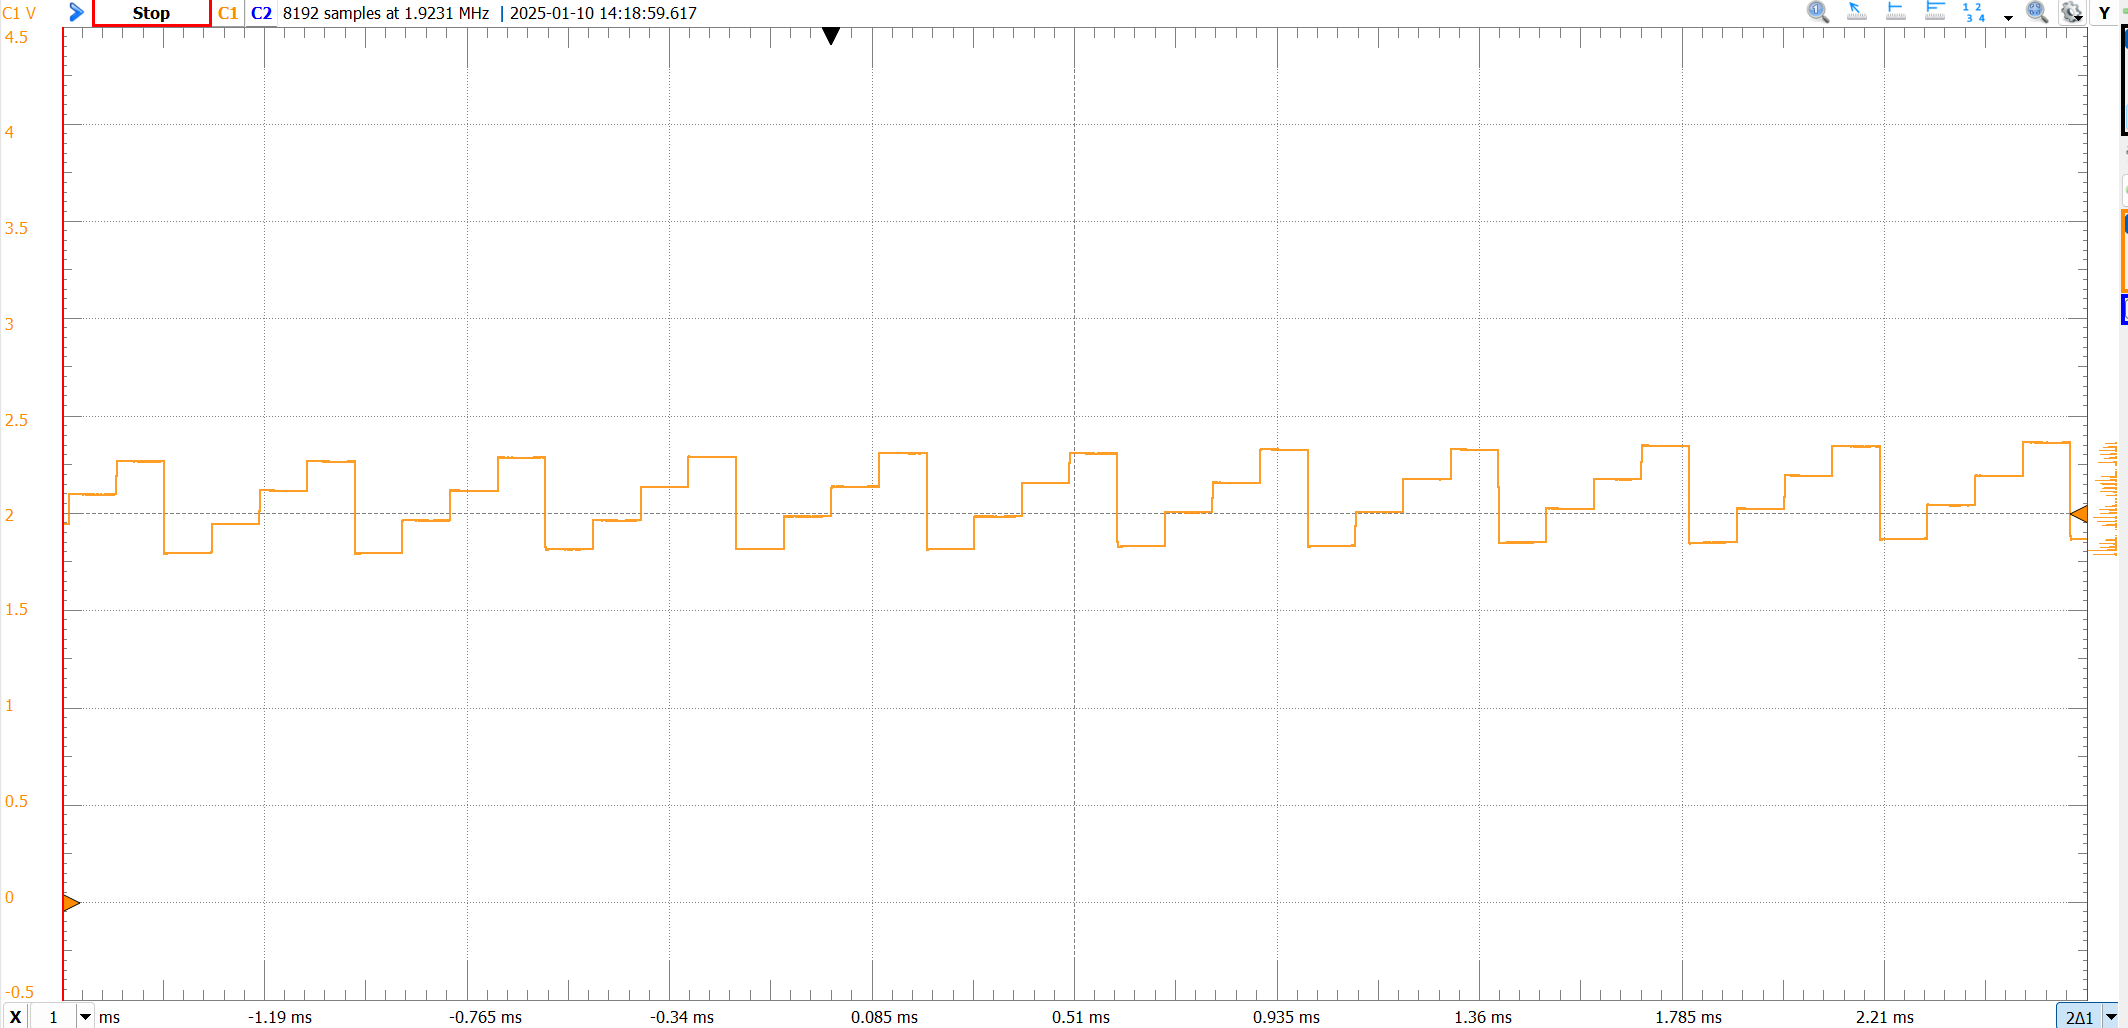
\includegraphics[width=0.75\linewidth]{img/Signal_07.png}
\end{figure}

\paragraph{Frequenzbereich}\mbox{}\\
Im Frequenzbereich des Signals können kaum sinnvolle Punkte erkannt werden, welche mit der Theorie übereinstimmen, da sich das Ausgangssignal ständig verändert, ändert sich auch das Diagramm im Frequenzbereich. Jedoch kann bei einer Frequenz von 0 Hz eine Spannung erkannt werden. Diese DC-Spannung stammt (laut Theorie) von der unteren Spiegelung des Eingangssignals bei der Samplingfrequenz (10 kHz - 10 kHz = 0 Hz). Theoretisch sollten sich weitere Punkte alle 10 kHz befinden, was allerdings nicht erkennbar ist.
\begin{figure}[h]
    \centering
    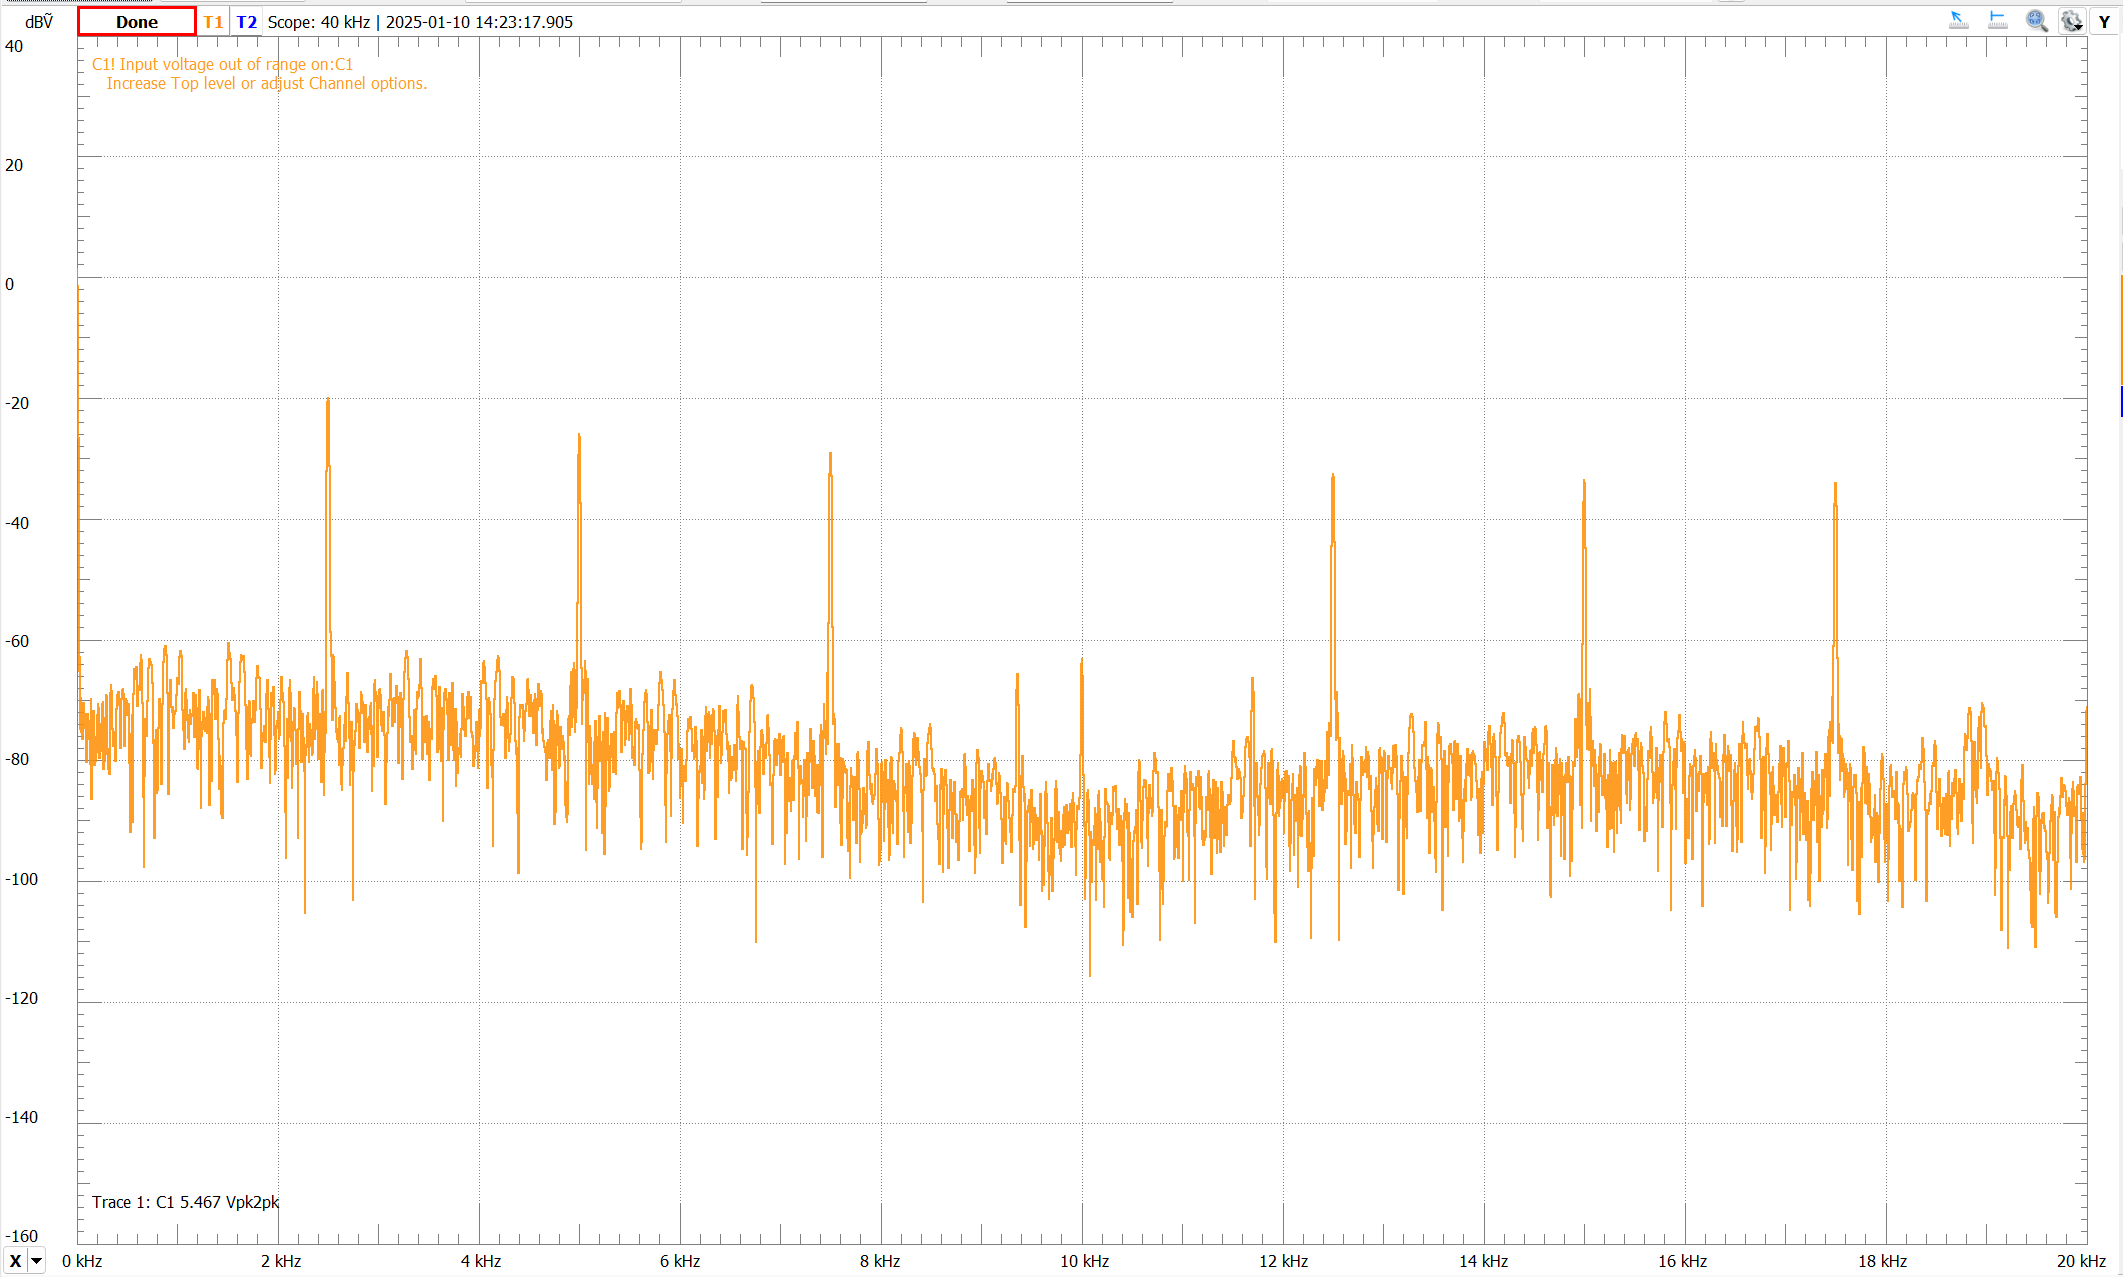
\includegraphics[width=0.75\linewidth]{img/Freq_07.png}
\end{figure}

\subsubsection{12kHz}
\paragraph{Zeitbereich}\mbox{}\\
Wie bei einer Eingangsfrequenz von 8 kHz ähnelt das Signal sehr dem Signal bei einer Eingangsfrequenz von 2 kHz. Dies liegt daran, dass das Signal durch den Aliasfehler als 2 kHz wahrgenommen wird.
\begin{figure}[h]
    \centering
    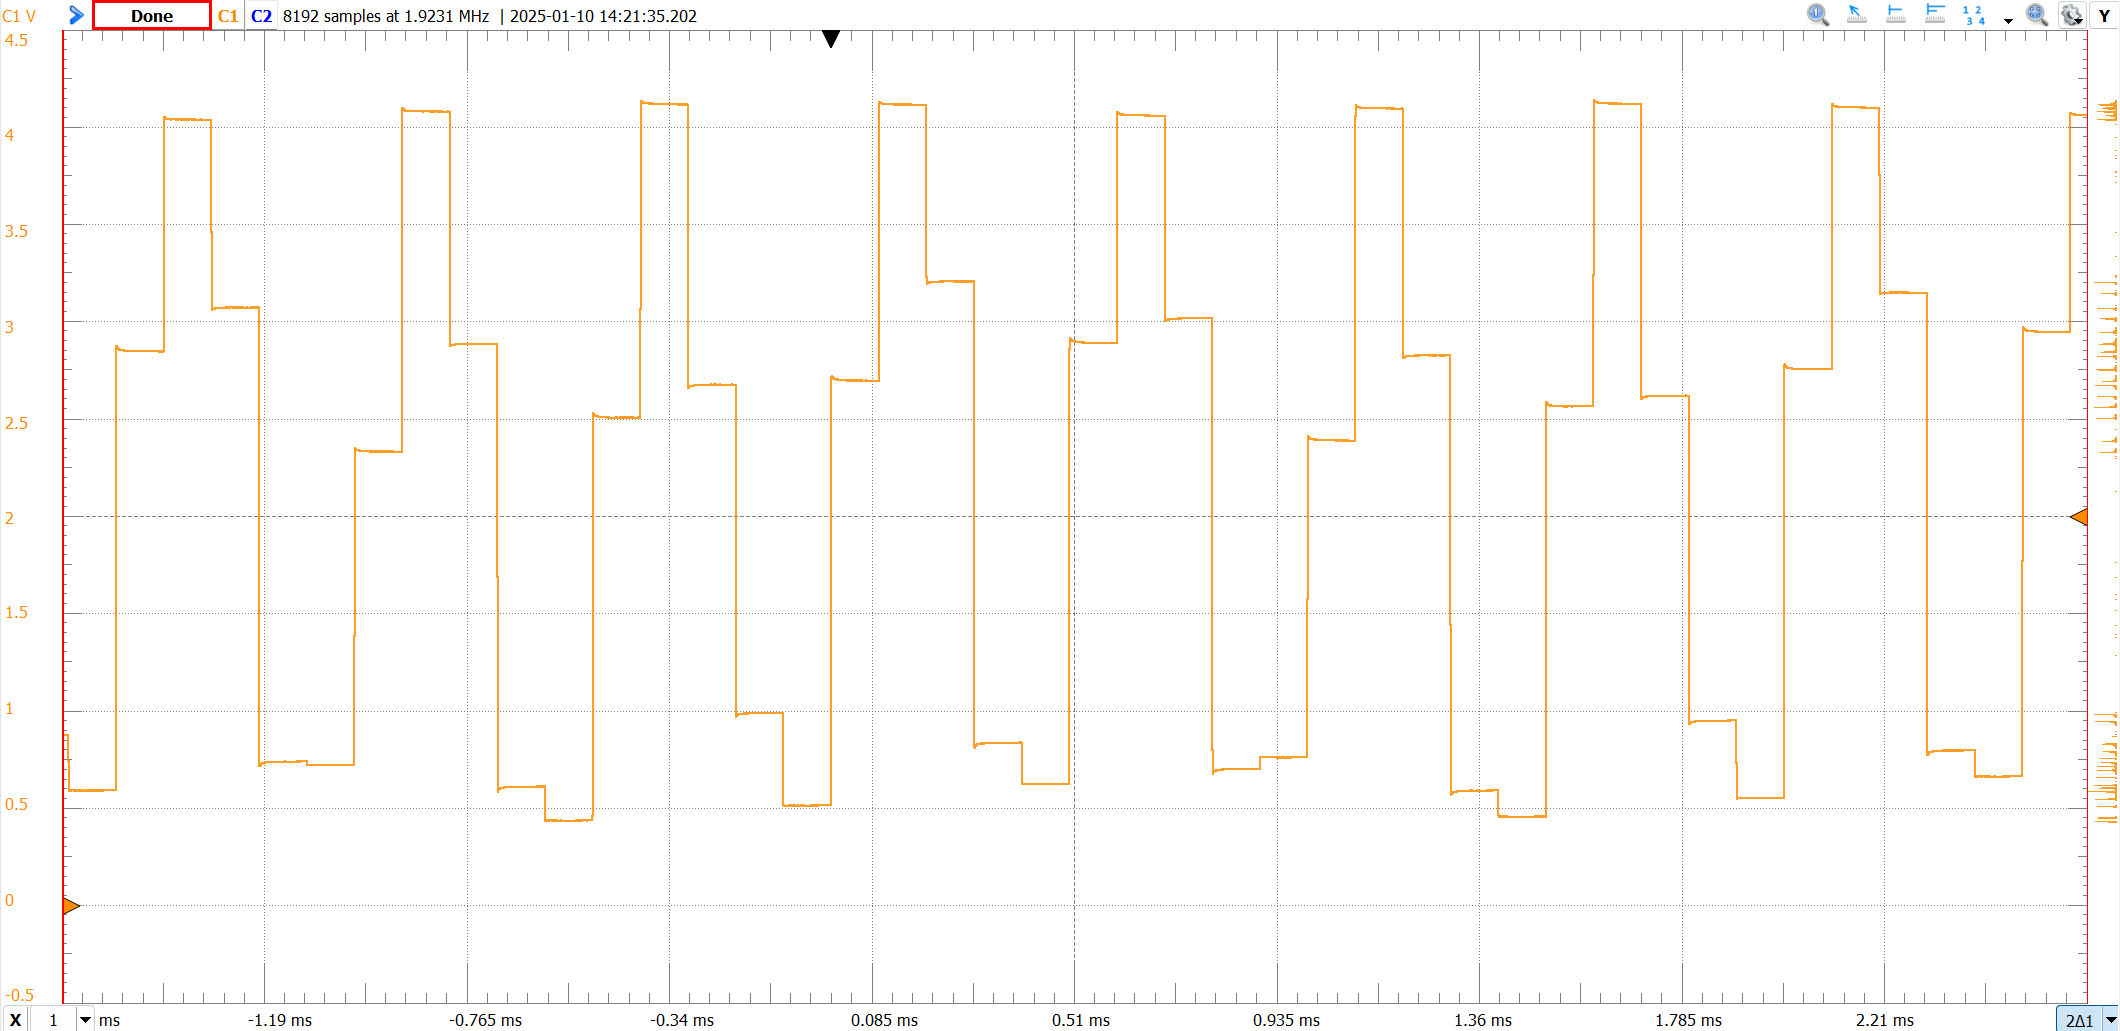
\includegraphics[width=0.8\linewidth]{img/Signal_08.png}
\end{figure}

\paragraph{Frequenzbereich}\mbox{}\\
Im Frequenzbereich des Signals kann erneut die Ähnlichkeit zu 2 kHz erkannt werden. Der Peak bei 2 kHz stammt von der unteren Spiegelung bei der Samplingfrequenz (10 kHz - 12 kHz = -2 kHz). Dabei werden negative Frequenzen als positive wahrgenommen, da sich bei ihnen der Sinus nur in die gegengesetzte Richtung drehen würde.
\begin{figure}[h]
    \centering
    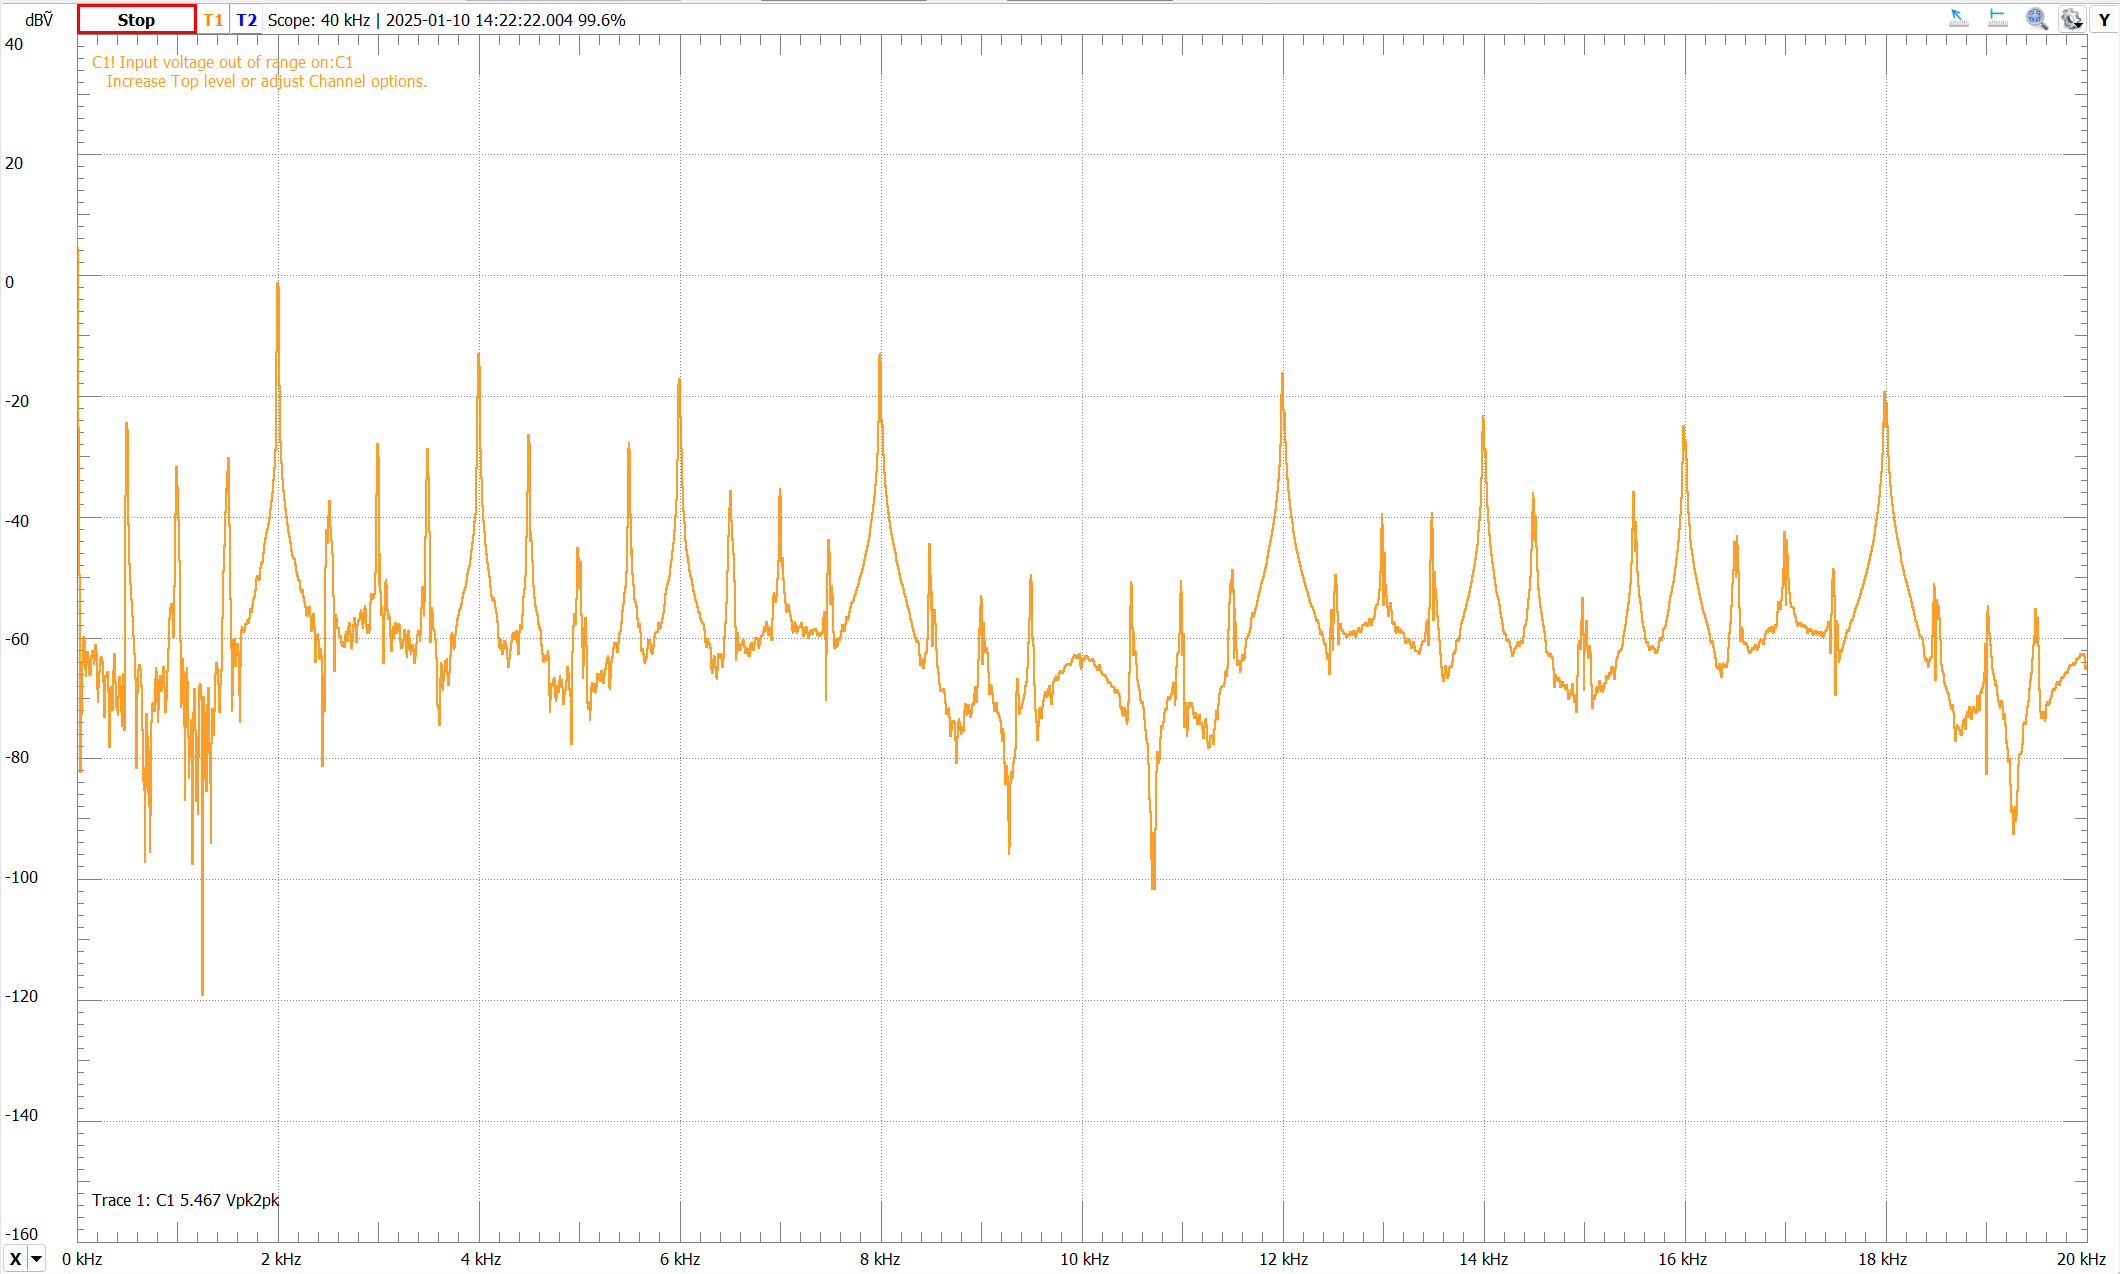
\includegraphics[width=0.8\linewidth]{img/Freq_08.png}
\end{figure}
\newpage
\subsection{Untersuchung der sinc()-Dämpfung}
\subsubsection{Aufgabenstellung}
In dieser Aufgabe soll die sinc()-Dämpfung eines 2 kHz-Signals bei 2 kHz und 8 kHz herausgemessen und mit der Theorie verglichen werden.

\subsubsection{Theorie}
Die Verstärkung (bzw. Dämpfung) der sinc()-Funktion kann über folgende Formel berechnet werden:
\begin{equation}
  a(f) := 20 \cdot \log \left( \frac{\sin \left( \pi \cdot \frac{f}{f_a} \right)}{\pi \cdot \frac{f}{f_a}} \right)
\end{equation}
dabei ist f die gesuchte Frequenz und $f_a$ die Samplingfrequenz, welche in diesem Fall 10 kHz beträgt. Beim Plotten dieser Funktion entsteht folgender Graph:
\begin{figure}[h]
    \centering
    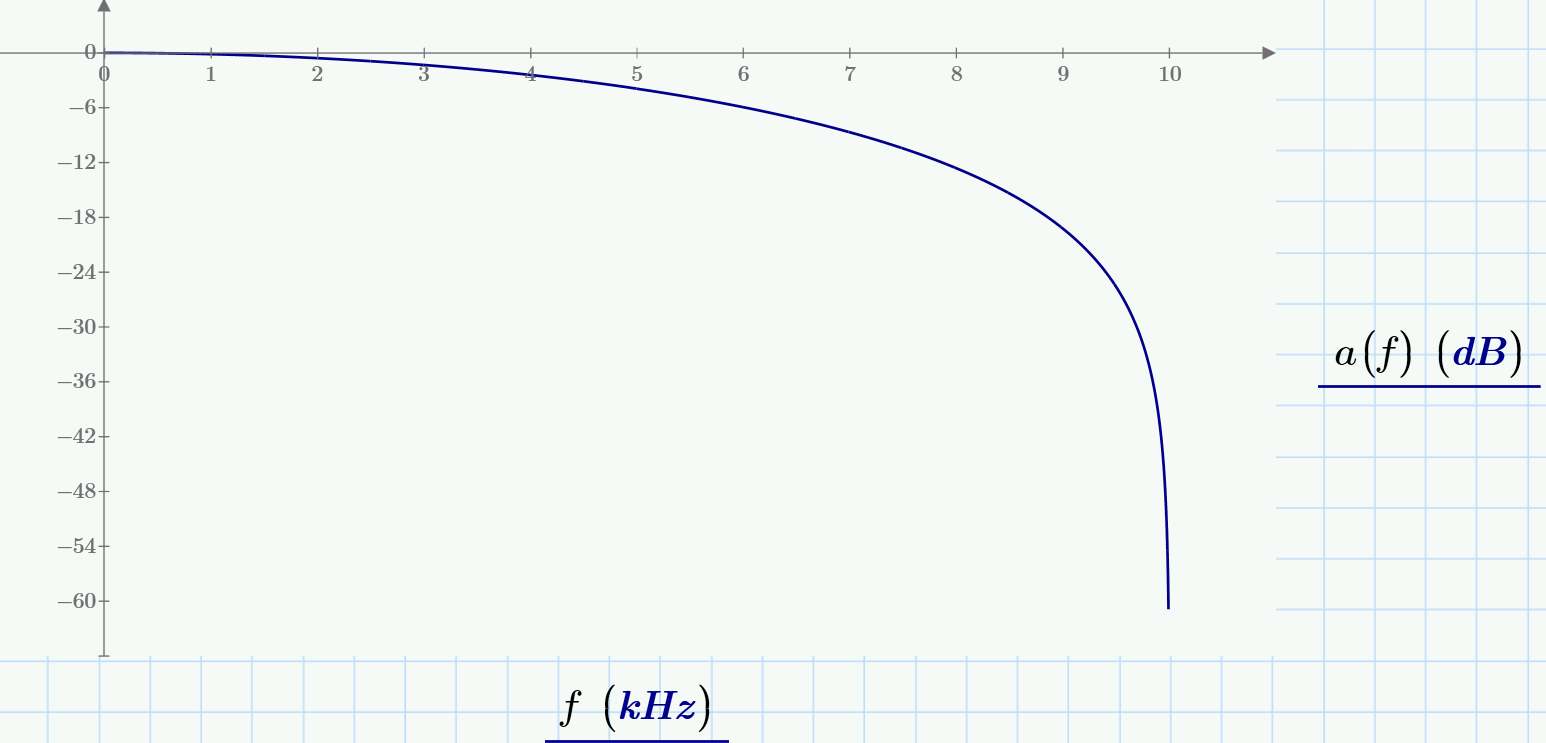
\includegraphics[width=0.6\linewidth]{img/graph_01.png}
\end{figure}
Aus diesem Graph kann ausgelesen werden, dass die Dämpfung bei einer Frequenz von 2 kHz -0.579 dB und bei einer Frequenz von 8 kHz -12.62 dB beträgt.
\subsubsection{Messung der Werte}
\begin{figure}[h]
    \centering
    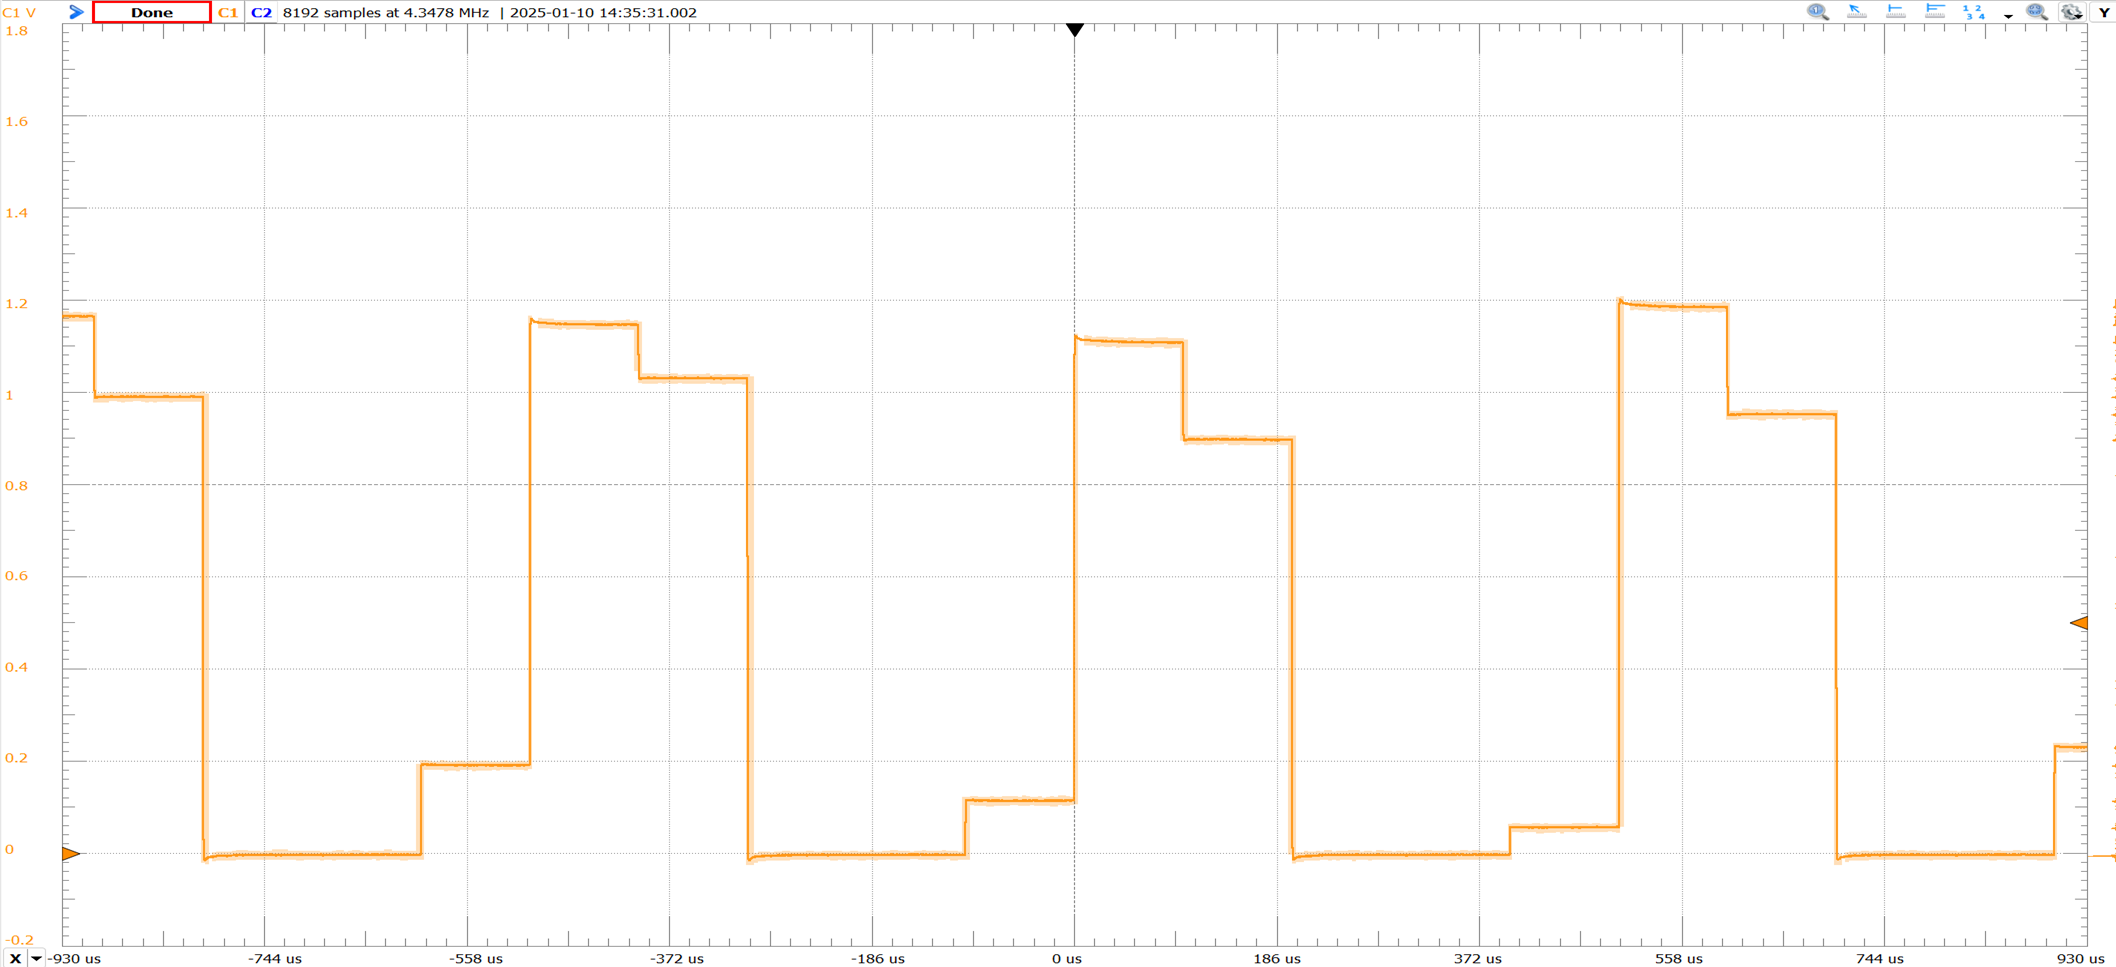
\includegraphics[width=0.7\linewidth]{img/Signal_09.png}
\end{figure}
Das gemessene Frequenzspektrum ist dem aus der vorherigen Aufgabe sehr ähnlich. Die Dämpfung bei einer Frequenz beträgt laut Messung ca. \textbf{-0.894 dB} und bei einer Frequenz von 8 kHz ca. \textbf{-11.49 dB}.

\subsubsection{Vergleich}
Wenn man die Werte der Theorie und der Messung vergleicht, sind diese sehr ähnlich. Die Dämpfung bei 2 kHz unterscheidet sich um 0.315 dB und bei 8 kHz nur um 1.13 dB. Diese Abweichungen stammen von möglichen Toleranzen der Frequenzen, was zur Folge hat, dass sich die sinc()-Funktion verzehrt. Aber auch die Auflösung des Analog Discoveries beeinflusst dies.
\newpage
\subsection{Aliassimulation}
\subsubsection{Aufgabenstellung}
In dieser Aufgabe soll eine Aliasspannung simuliert werden, indem eine Sinusspannung mit 8 kHz eingespeist wird. Um einen besseren Vergleich zu ermöglichen, soll dies zuerst ohne den Antialiasingfilter (X1 aus) und anschließend mit dem Antialiasingfilter (X1 ein) aufgenommen werden. Dabei sollen Änderungen im Nutzbereich (0 ... fa/2) beschrieben werden und das Ergebnis sowohl im Zeit- als auch im Frequenzbereich mit der Theorie verglichen werden.

\subsubsection{Theorie}
Die Dämpfung eines Tiefpasses 1. Ordnung kann mit folgender Formel ausgerechnet werden:
\begin{equation}
    H_{TP}(f) := \frac{1}{\sqrt{1 + \left( \frac{f}{f_g} \right)^2}}
    \label{eq:placeholder}
\end{equation}
Dabei ist f die Signalfrequenz und $f_g$ die Grenzfrequenz des Tiefpasses. Wenn diese Funktion geplottet wird, entsteht folgender Graph:\\
\begin{figure}[h]
    \centering
    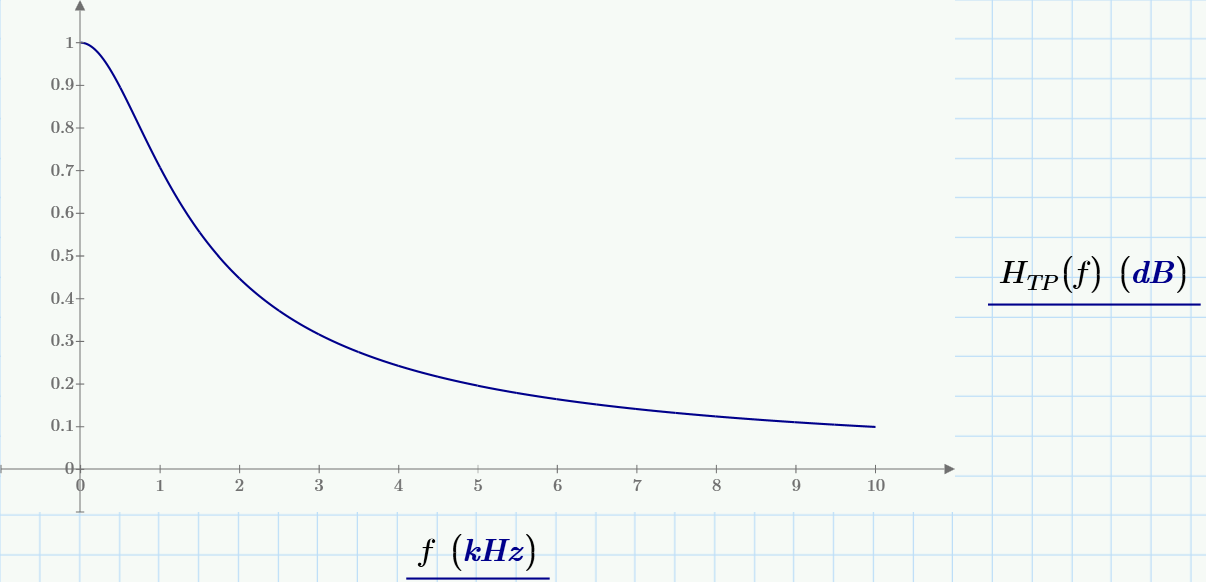
\includegraphics[width=0.8\linewidth]{img/graph_02.png}
\end{figure}\\
Aus diesem Graph kann herausgelesen werden, dass der Tiefpass ein Signal mit einer Frequenz von 2 kHz mit \textbf{0.447 (-7 dB)} und einer Frequenz von 8 kHz mit \textbf{0.124 (-18.129 dB)} dämpft.\\
\newpage
\subsubsection{Messung ohne Antialiasingfilter}
\paragraph{Zeitbereich}\mbox{}\\
Die Form des erhaltenen Signals im Zeitbereich ist ähnlich wie in der vorherigen Aufgabe, bei der auch ein Eingangssignal mit 2 kHz eingespeist wurde. Allerdings ist das Signal kleiner als zuvor. (Dies sollte eigentlich nicht der Fall sein. Es besteht die Annahme, dass eine falsche Eingangsspannung eingestellt wurde.)
\begin{figure}[h]
    \centering
    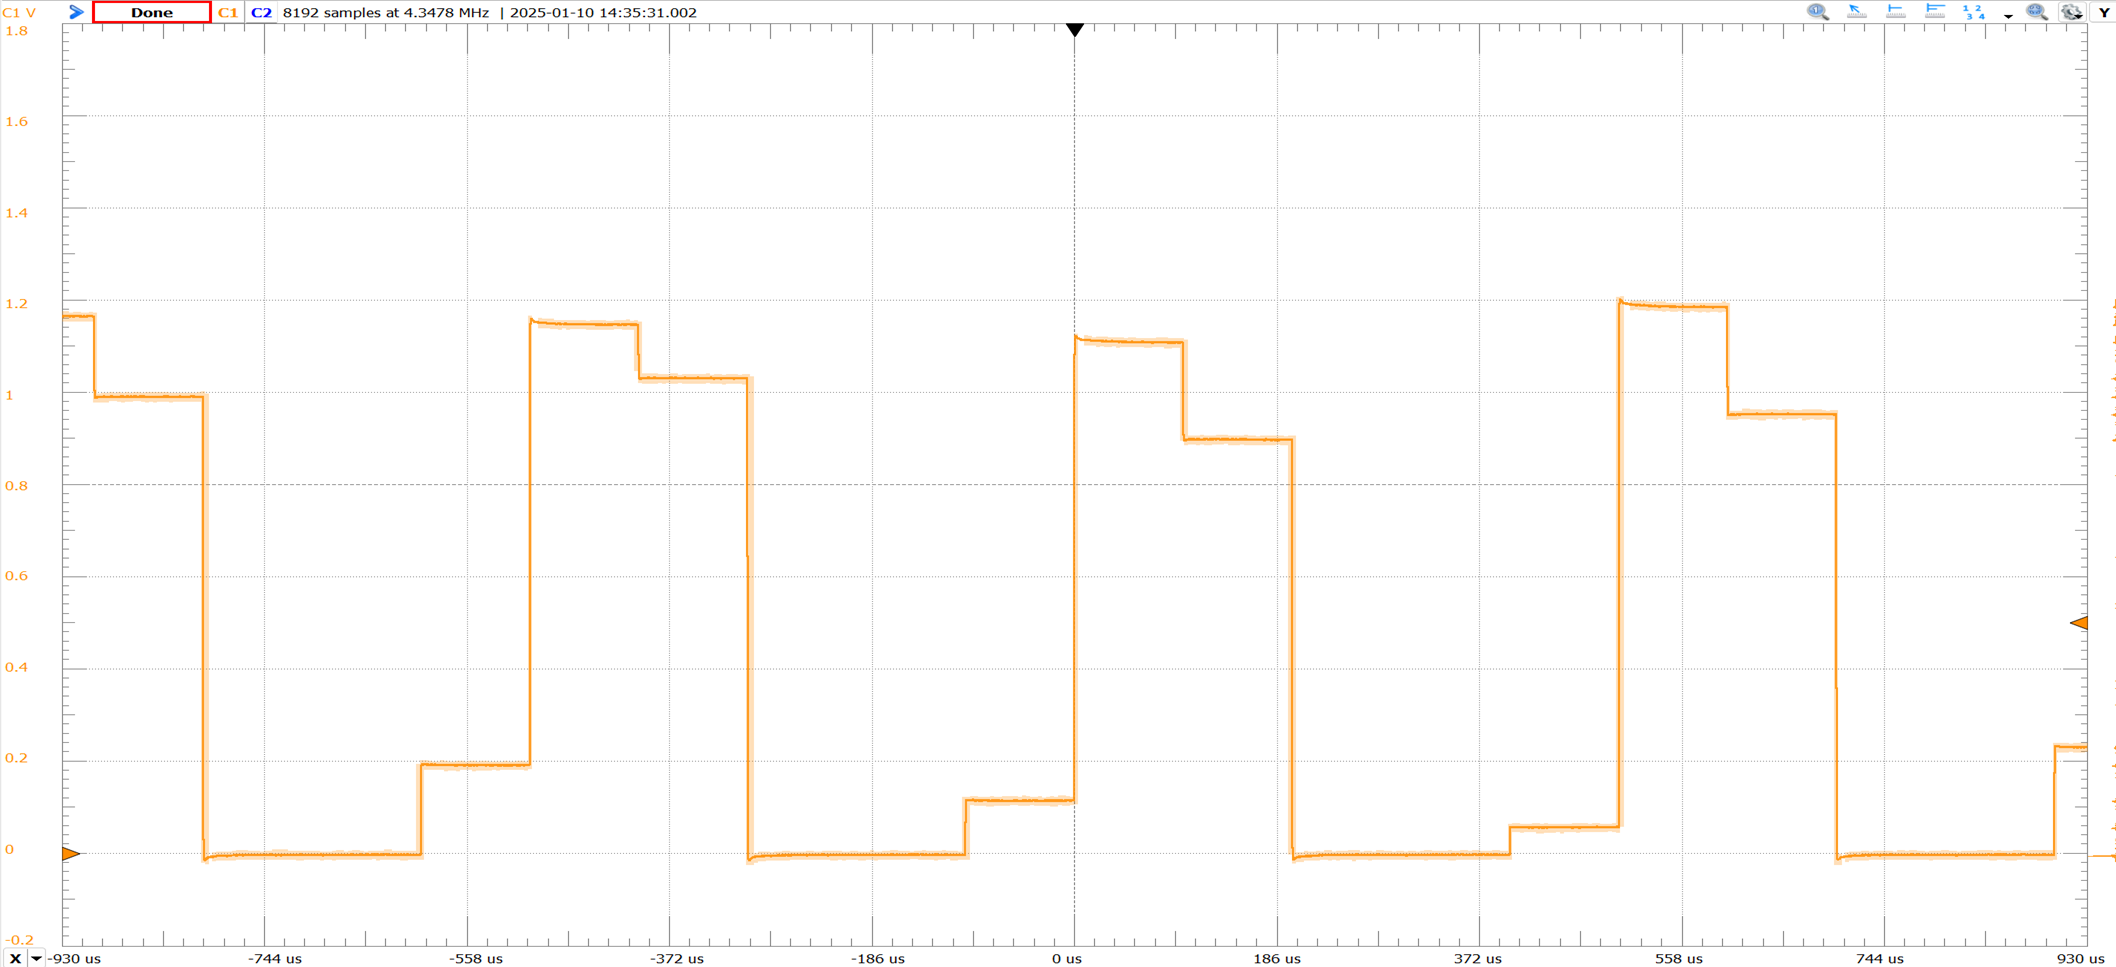
\includegraphics[width=0.8\linewidth]{img/Signal_09.png}
\end{figure}

\paragraph{Frequenzbereich}\mbox{}\\
Wie im Zeitbereich ist das Signal auch im Frequenzbereich dem vorherigen 2 kHz Signal sehr ähnlich.
\begin{figure}[h]
    \centering
    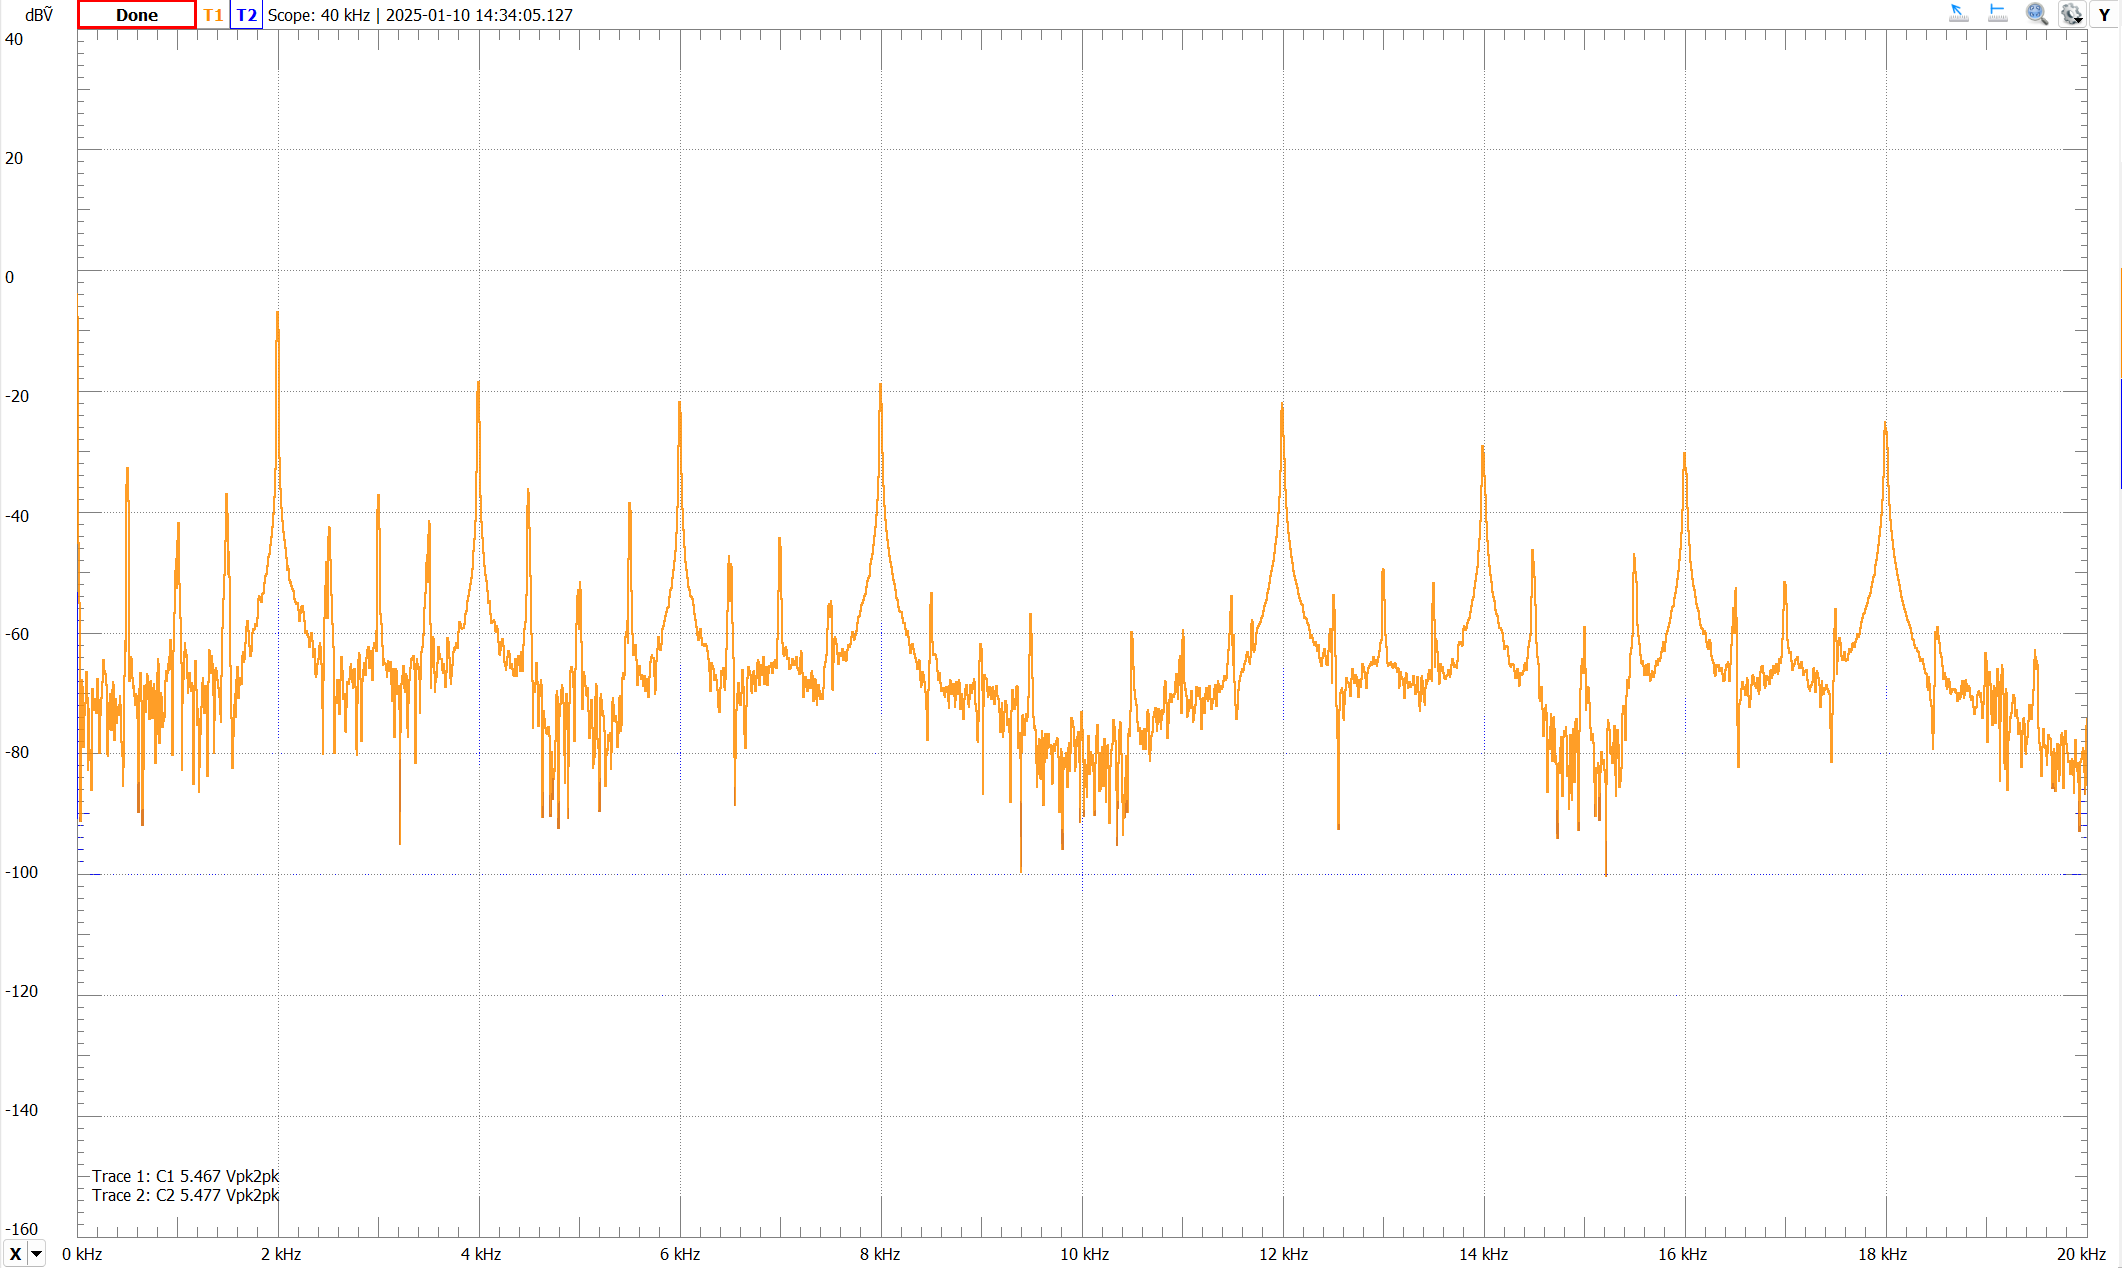
\includegraphics[width=0.8\linewidth]{img/Freq_09.png}
\end{figure}

\newpage
\subsubsection{Messung mit Antialiasingfilter}
Im Vergleich zum vorherigen Signal ist die Spannung des Signals kleiner. Grund dafür ist, dass der Tiefpass die Spannungen dämpft. Zudem erinnert die Form des Signals mehr an einen Sinus als zuvor.
\paragraph{Zeitbereich}\mbox{}\\
\begin{figure}[h]
    \centering
    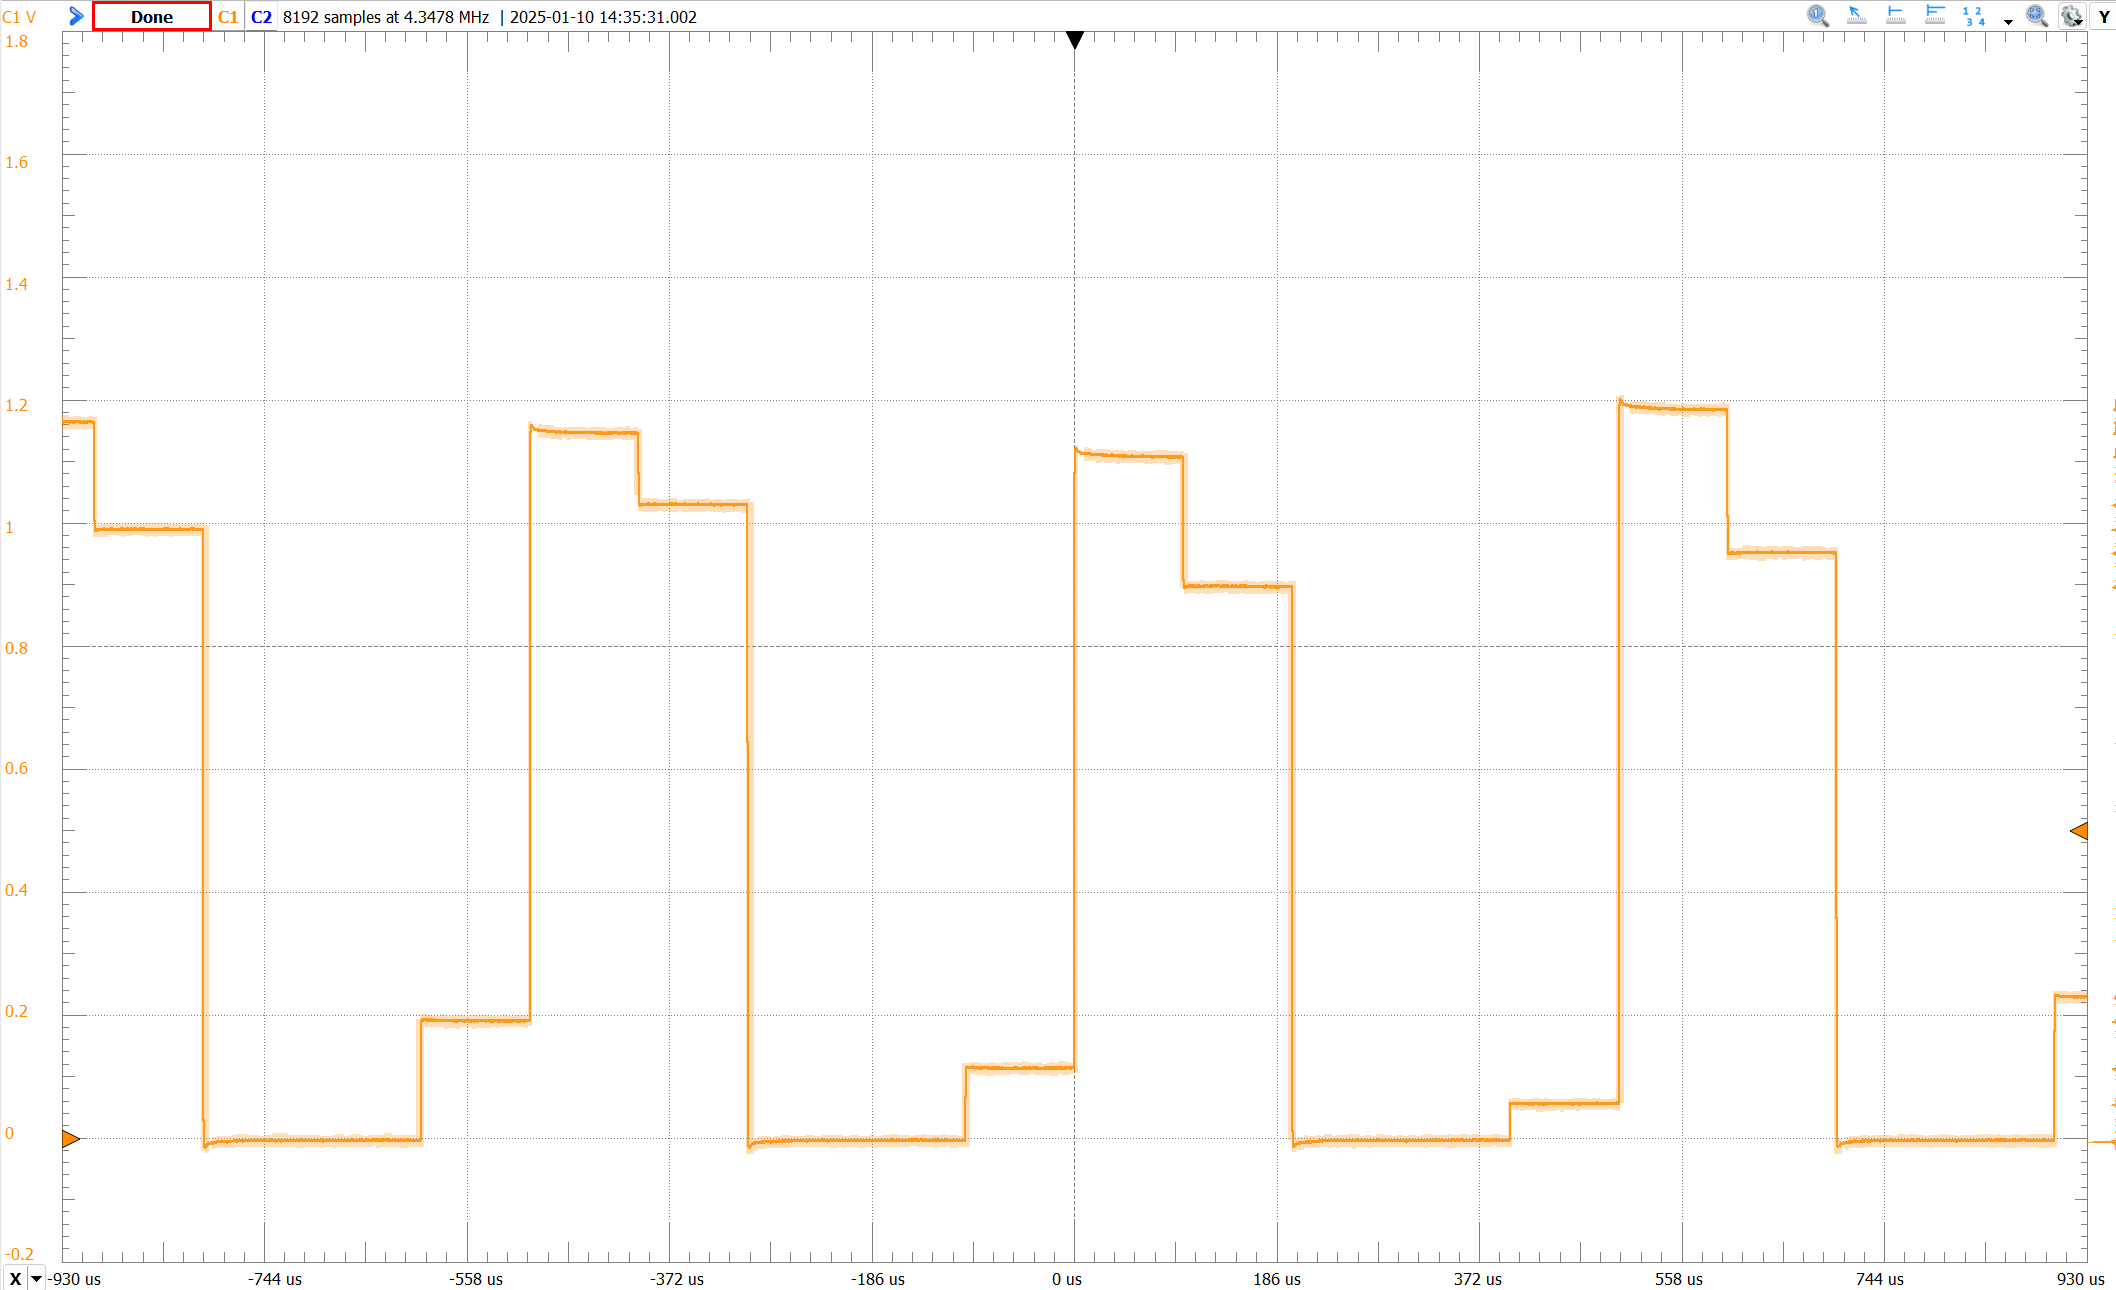
\includegraphics[width=0.6\linewidth]{img/Signal_10.png}
\end{figure}

\paragraph{Frequenzbereich}\mbox{}\\
Der Frequenzbereich des gefilterten Signals unterscheidet sich deutlich von vorherigen. Hier ist klar erkennbar, dass viele ungewollte Frequenzen entfernt wurden, da hauptsächlich die zwei Peaks bei 2 kHz und 8 kHz erkennbar sind. Dabei hat der Peak bei 2 kHz einen Wert von ca. -22 dB und bei 8kHz ca. -32 dB.
\begin{figure}[h]
    \centering
    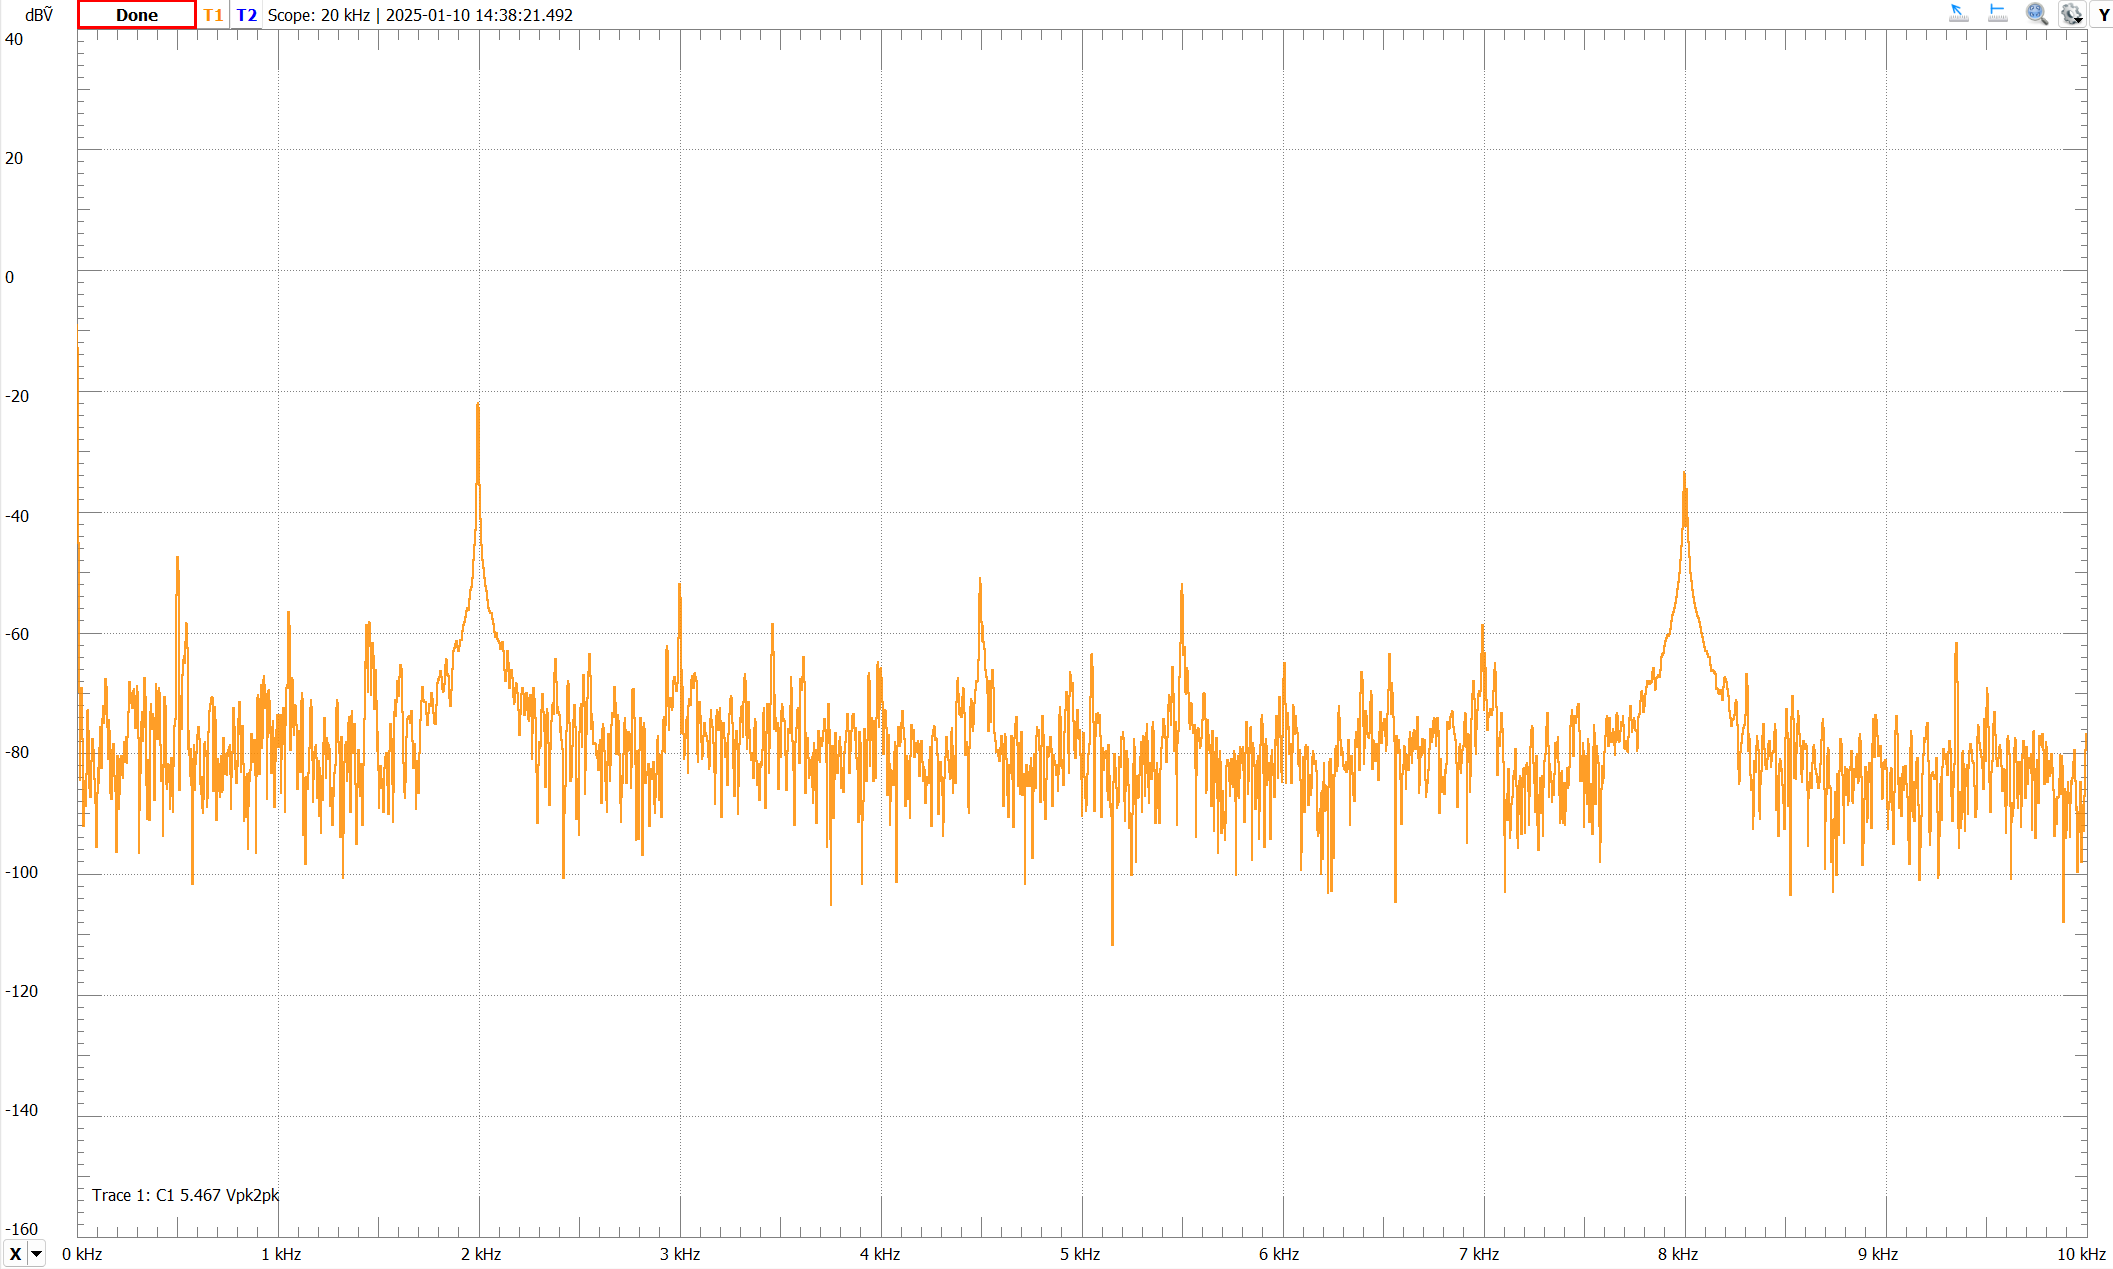
\includegraphics[width=0.6\linewidth]{img/Freq_10.png}
\end{figure}

\subsubsection{Vergleich}
Die theoretischen Werte unterscheiden sich stark von den Messergebnissen. Wie schon beschrieben, wird vermutet, dass eine falsche Eingangsspannung eingestellt wurde, da ohne Filter ein seltsames Ergebnis gemessen wurde. Kleine Abweichungen wären durch Bauteilungenauigkeiten oder andere Toleranzen des Systems normal, aber die starken Abweichungen des Ergebnisses weisen auf ein größeres Problem bei der Messung.

\newpage
\section{Übung 2: IIR-TP-Filter 1. Ordnung}
\subsection{Programmierung des IIR-TP}
\subsubsection{Aufgabenstellung}
In dieser Aufgabe soll der IIR-Tiefpass-Filter 1. Ordnung in der ISR implementiert werden. Dafür sollen folgende Koeffiziente verwendet werden:
\begin{math}
    b_0=0.1\\
    a_1=0.9
\end{math}
Diese müssen in die allgemeine Formel des IIR-Filters eingesetzt werden.
\begin{equation}
    y(n) = \sum_{k=0}^{M} b_k \cdot x(n-k) - \sum_{j=1}^{N} a_j \cdot y(n-j)
    \label{eq:iir_filter}
\end{equation}
Für einen Filter 1. Ordnung lautet die benötigte Formel:
\begin{equation}
    y(n) = b_0 \cdot x(n) + y(n-1) \cdot a_1
\end{equation}

\subsubsection{Programmcode}
Der Programmcode wurde mit Floatingpoint-Zahlen ausprogrammiert.
\begin{minted}{c}
ISR(TIMER0_COMP_vect)                      //fa=10kHz --> T=100us
{ 
    ue=ADCH;                  //Einlesen des Samples
    ADCSRA|=(1<<ADSC);        //Start der neuen Messung
    
    float x_neu = (float)ue;  //ADC-Wert in Float umwandeln
    
    //  u(n) = x(n) * b0     + y(n-1) * a1
    float y_neu = x_neu * b0 + y_alt  * a1;
    
    ua = (unsigned char)y_neu; //float zu char
    
    y_alt = y_neu;             //Speicher für nächste Rechnung

    PORTC=ua;                  //Ausgabe des Samples
}
\end{minted}
\newpage
\subsection{Frequenzgang}
\subsubsection{Aufgabenstellung}
In dieser Aufgabe soll der Frequenzgang des ausprogrammierten IIR-Tiefpasses überprüft werden. Dafür soll der Netzwerk-Analysator des Analog Discoverys verwendet werden. Dieser soll einen DC-Offset von 2 V und eine Amplitude von 1 V besitzen.

\subsubsection{Messung}
Am folgenden Frequenzgang ist klar erkennbar, dass es sich um einen Tiefpass 1. Ordnung handelt. Es handelt sich um einen Tiefpass, da die Verstärkung bei niedrigen Frequenzen fast konstant verläuft und dann abfällt.
\begin{figure}[h]
    \centering
    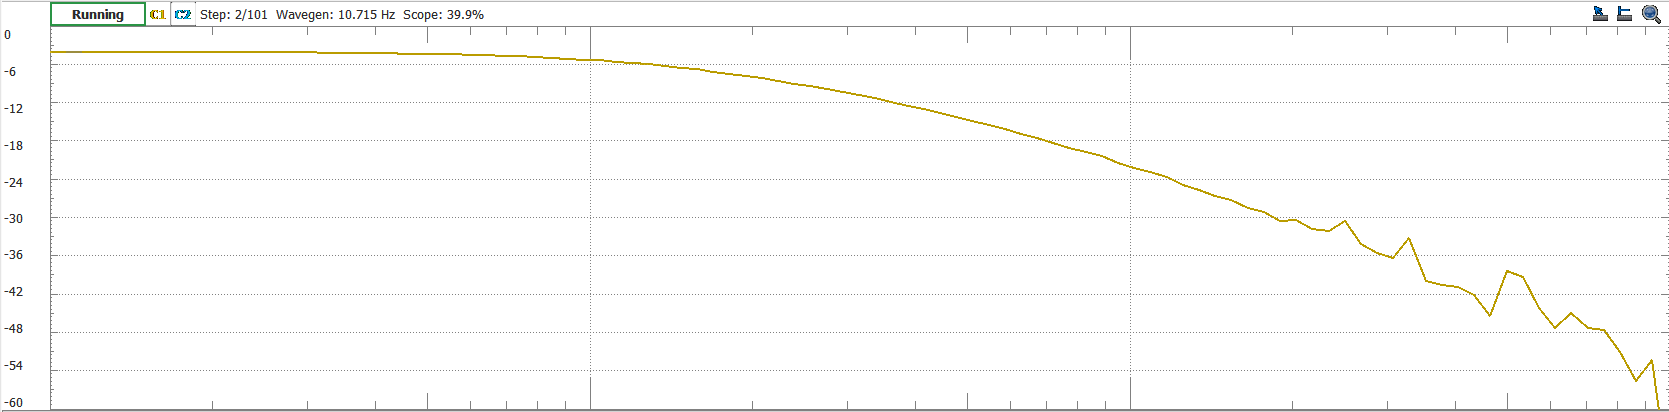
\includegraphics[width=0.5\linewidth]{img/Bode_01.png}
\end{figure}
\textit{Der Graph läuft von 10Hz bis 10kHz (x-Achsenbeschriftung wurde im Screenshot abgehackt)}\\
Da die Verstärkung bei niedrigen Frequenzen ca. -3.5 dB groß ist, hat die Grenzfrequenz eine Verstärkung von -6.5 dB. Laut Graph ist dies bei ca. 150 Hz. Da die Verstärkung bei 200 Hz ca. -7.5 dB und bei 2 kHz ca. -30 dB groß ist, ist die Verstärkung um 22.5 dB gefallen (-20 dB / Dekade). Da dies ungefähr einem Abfall von 20 dB pro Dekade entspricht, handelt es sich um einen Tiefpass 1. Ordnung.

\subsection{Simulation des Filters}
\subsubsection{Aufgabenstellung}
In dieser Aufgabe soll das IIR-TP-Filter in Matlab simuliert werden. Dafür soll der freqz()-Befehl eingesetzt werden. Aus dem entstandenen Frequenzgang soll die Grenzfrequenz und Flankensteilheit ausgemessen werden.

\subsubsection{Matlab-Code}
\begin{minted}{matlab}
%Koeffizienten
b0 = 0.1;
a1 = 0.9;

b = [b0];     %Zähler
a = [1, -a1]; %Nenner

%Frequenzgang
[H, f] = freqz(b, a, 2^16, 10000); %2^16 Punkte, Sample 10 kHz

%Plotten
semilogx(f, 20*log10(abs(H)));
xlabel('Frequenz [Hz]')
ylabel('Verstärkung [dB]')
grid on;
title('Frequenzgang');
\end{minted}
\newpage
\subsubsection{Frequenzgang}
Der entstehende Frequenzgang stellt einen Tiefpass dar. Dieser hat bei niedrig eine Verstärkung von 0 dB und filter hohe Frequenzen weg.
\begin{figure}[h]
    \centering
    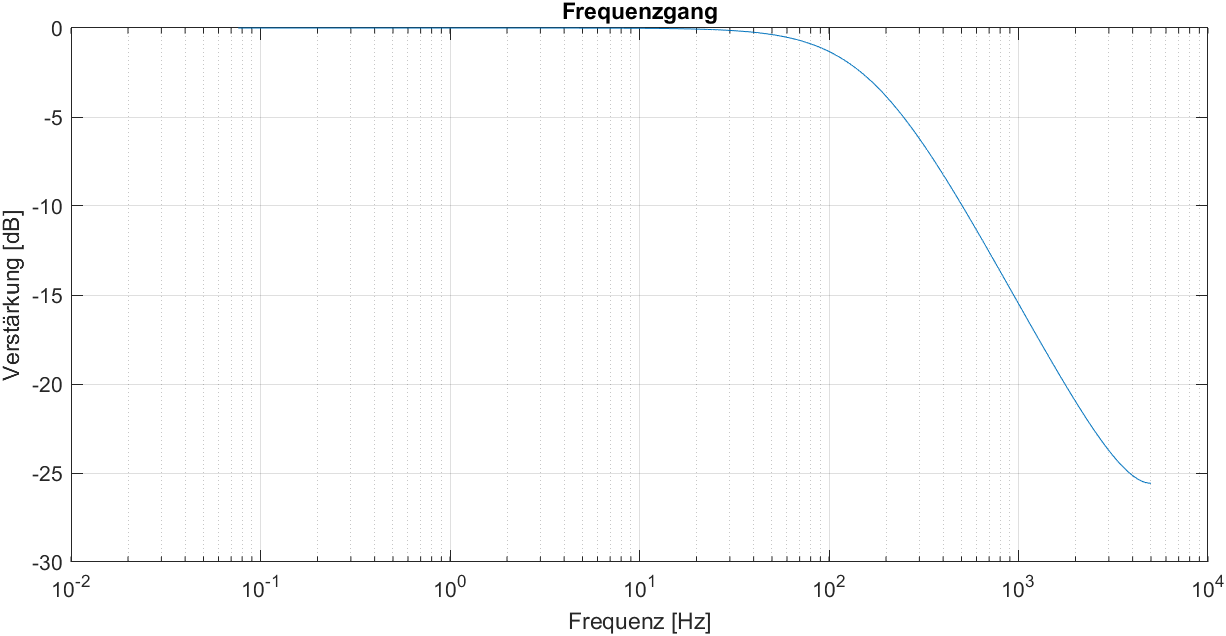
\includegraphics[width=0.8\linewidth]{img/Bode_04.png}
\end{figure}

\subsubsection{Messung der Grenzfrequenz}
Die Grenzfrequenz (Punkt bei -3 dB) liegt laut Simulation bei einer Frequenz von ca. 168.762 Hz.
\begin{figure}[h]
    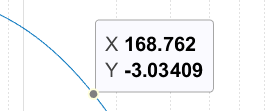
\includegraphics[width=0.25\linewidth]{img/Bode_Mess_01.png}
\end{figure}

\subsubsection{Messung der Flankensteilheit}
Um die Flankensteilheit zu messen, müssen zwei Punkte bekannt sein. Da durch die Messung der Grenzfrequenz schon ein Punkt vorhanden ist, muss nur noch ein Punkt erfasst werden. Dieser liegt eine Dekade nach dem ersten Punkt, also bei 1687.62 Hz. Dort liegt die Verstärkung bei ca. -19.6181 dB. Somit liegt die Differenz bei ca. 16.6171 dB. Ein gewöhnlicher Tiefpass 1. Ordnung sollte einen Abfall von -20 dB / Dekade haben. Die Abweichung des Messergebnisses stammt von der nahen Messung an der Grenzfrequenz, bei welcher der Tiefpass noch nicht linear abfällt.
\begin{figure}[h]
    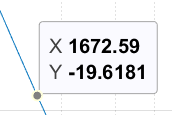
\includegraphics[width=0.25\linewidth]{img/Bode_Mess_02.png}
\end{figure}

\newpage
\section{Übung 3 - IIR-HP-Filter 2. Ordnung}
\subsection{Simulation des IIR-HP-Filters}
\subsubsection{Aufgabenstellung}
In dieser Aufgabe soll Matlab benutzt werden, um einen IIR-HP-Filter der 2. Ordnung zu entwerfen. Dieser soll eine Grenzfrequenz von 1000 Hz haben. Nachdem der Filter entworfen wurde, soll der Frequenzgang dessen untersucht werden.

\subsubsection{Entwurf des Filters}
\begin{minted}{matlab}
fc = 1000;  %Grenzfrequenz = 1kHz
fs = 10000; %Samplefrequenz = 10kHz

[b,a] = butter(2,fc/(fs/2), "high"); %Faktoren des Filter bestimmen

freqz(b,a,[],fs) %Frequenzgang berechnen

%Faktoren ausgeben
a1 = a(2)
a2 = a(3)

b0 = b(1)
b1 = b(2)
b2 = b(3)

%Frequenzgang plotten
subplot(2,1,1)
ylim([-100 20])
\end{minted}

\begin{figure}[h]
    \centering
    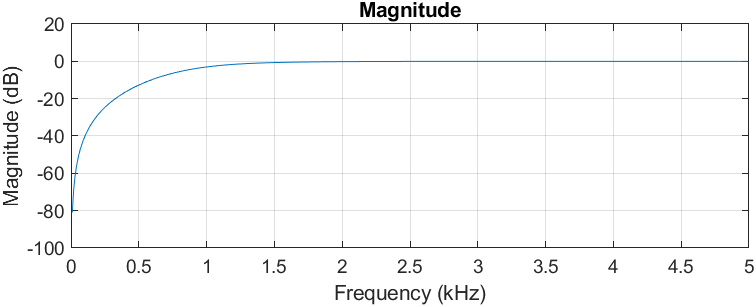
\includegraphics[width=0.7\linewidth]{img/Bode_02.png}
    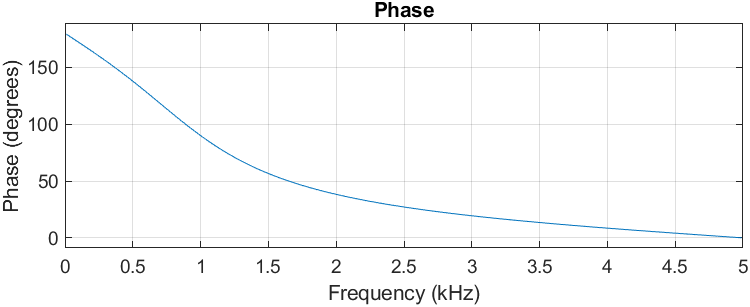
\includegraphics[width=0.7\linewidth]{img/Bode_03.png}
\end{figure}
\newpage
\subsection{Umwandlung in 16Bit unsigned Werte}
\subsubsection{Aufgabenstellung}
In dieser Aufgabe sollen die berechneten Koeffizienten als 16-Bit unsigned Werte exportiert werden, um sie auf der Megacard zu implementieren.

\subsubsection{Matlab-Code}
Der folgende Matlab-Code wandelt die dezimalen Koeffizienten in den benötigten Datentyp um. Dabei wurden sie mit 256 multipliziert, damit die Werte auf der Megacard die uint16-Größe nicht überschreiten. Die Formel des IIR-Filters wurde umgewandelt, damit alle eingegebenen Konstanten positiv sind.

\begin{minted}{matlab}
%Faktoren ausgeben
a1 = round(a(2) * 256)
a2 = round(a(3) * 256)

b0 = round(b(1) * 256)
b1 = round(b(2) * 256)
b2 = round(b(3) * 256)
\end{minted}

\subsubsection{Umformung der IIR-Formel}
In der folgenden Umformung wird die Gleichung des IIR-Filters so angepasst, dass keine negativen Koeffizienten mehr vorhanden sind.
\begin{figure}[h]
    \centering
    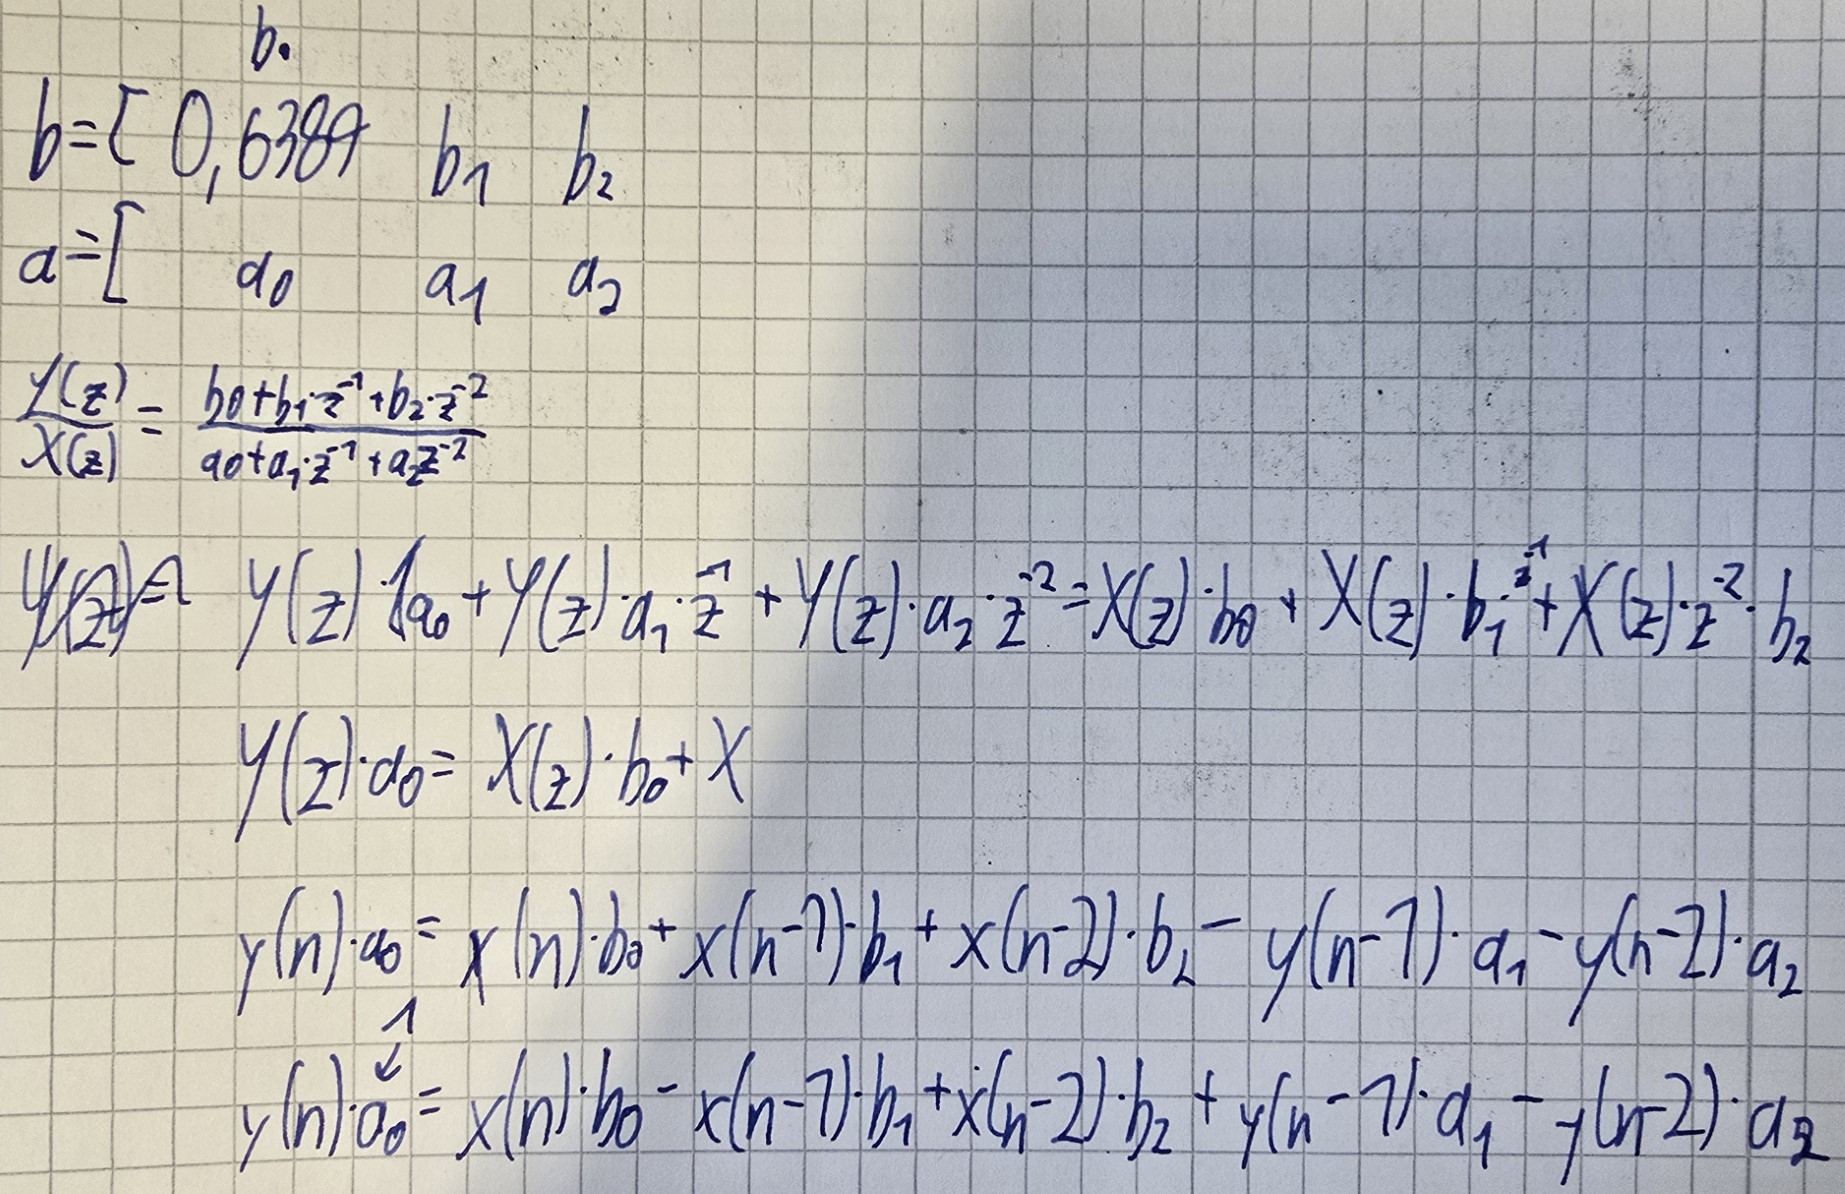
\includegraphics[width=0.8\linewidth]{img/Formel_01.jpg}
\end{figure}
\newpage
\subsection{Implementierung auf der Megacard}
\subsubsection{Aufgabenstellung}
In dieser Aufgabe sollen die exportierten uint16-Koeffizienten benutzt werden, um den HP-Filter auf der Megacard zu implementieren.

\subsubsection{Programmcode}
\begin{minted}{c}
ISR(TIMER0_COMP_vect)   //fa=10kHz --> T=100us
{ 
    ue=ADCH;			//Einlesen des Samples
    ADCSRA|=(1<<ADSC);  //Start der neuen Messung
 
    ua     = (uint16_t)(164*ue + 164 * x[1] + 293 * y[0] -106 * y[1] - 327 * x[0])>>8; //Wert ausrechnen
    //x-Werte zeitlich verschieben
    x[1] = x[0];
    x[0] = ue;

    //y-Werte zeitlich verschieben
    y[1] = y[0];
    y[0] = ua;

    PORTC=ua;         //Ausgabe des Samples
}
\end{minted}

\subsection{Messung des Frequenzganges}
\subsubsection{Aufgabenstellung}
In dieser Aufgabe soll die Implementierung des HP-Filters auf der Megacard getestet werden, indem der Frequenzgang aufgenommen wird.

\subsubsection{Bearbeitung}
Leider ergab die Implementierung des Codes keinen sauberen Frequenzgang. Am entstandenen Frequenzgang konnten zudem keine Hochpasscharakteristiken festgestellt werden. Es wurde versucht, den Fehler zu finden und zu beheben, aber dies hatte keinen Erfolg.

\section{Übung 4 - FIR-Filter}
Aus zeitlichen Gründen wurde diese Übung nicht behandelt.

\end{document}